\section{Assumptions}
\label{sec:assumptions}
\begin{figure}[htb]
\centering
%\subfloat[side view]{
%	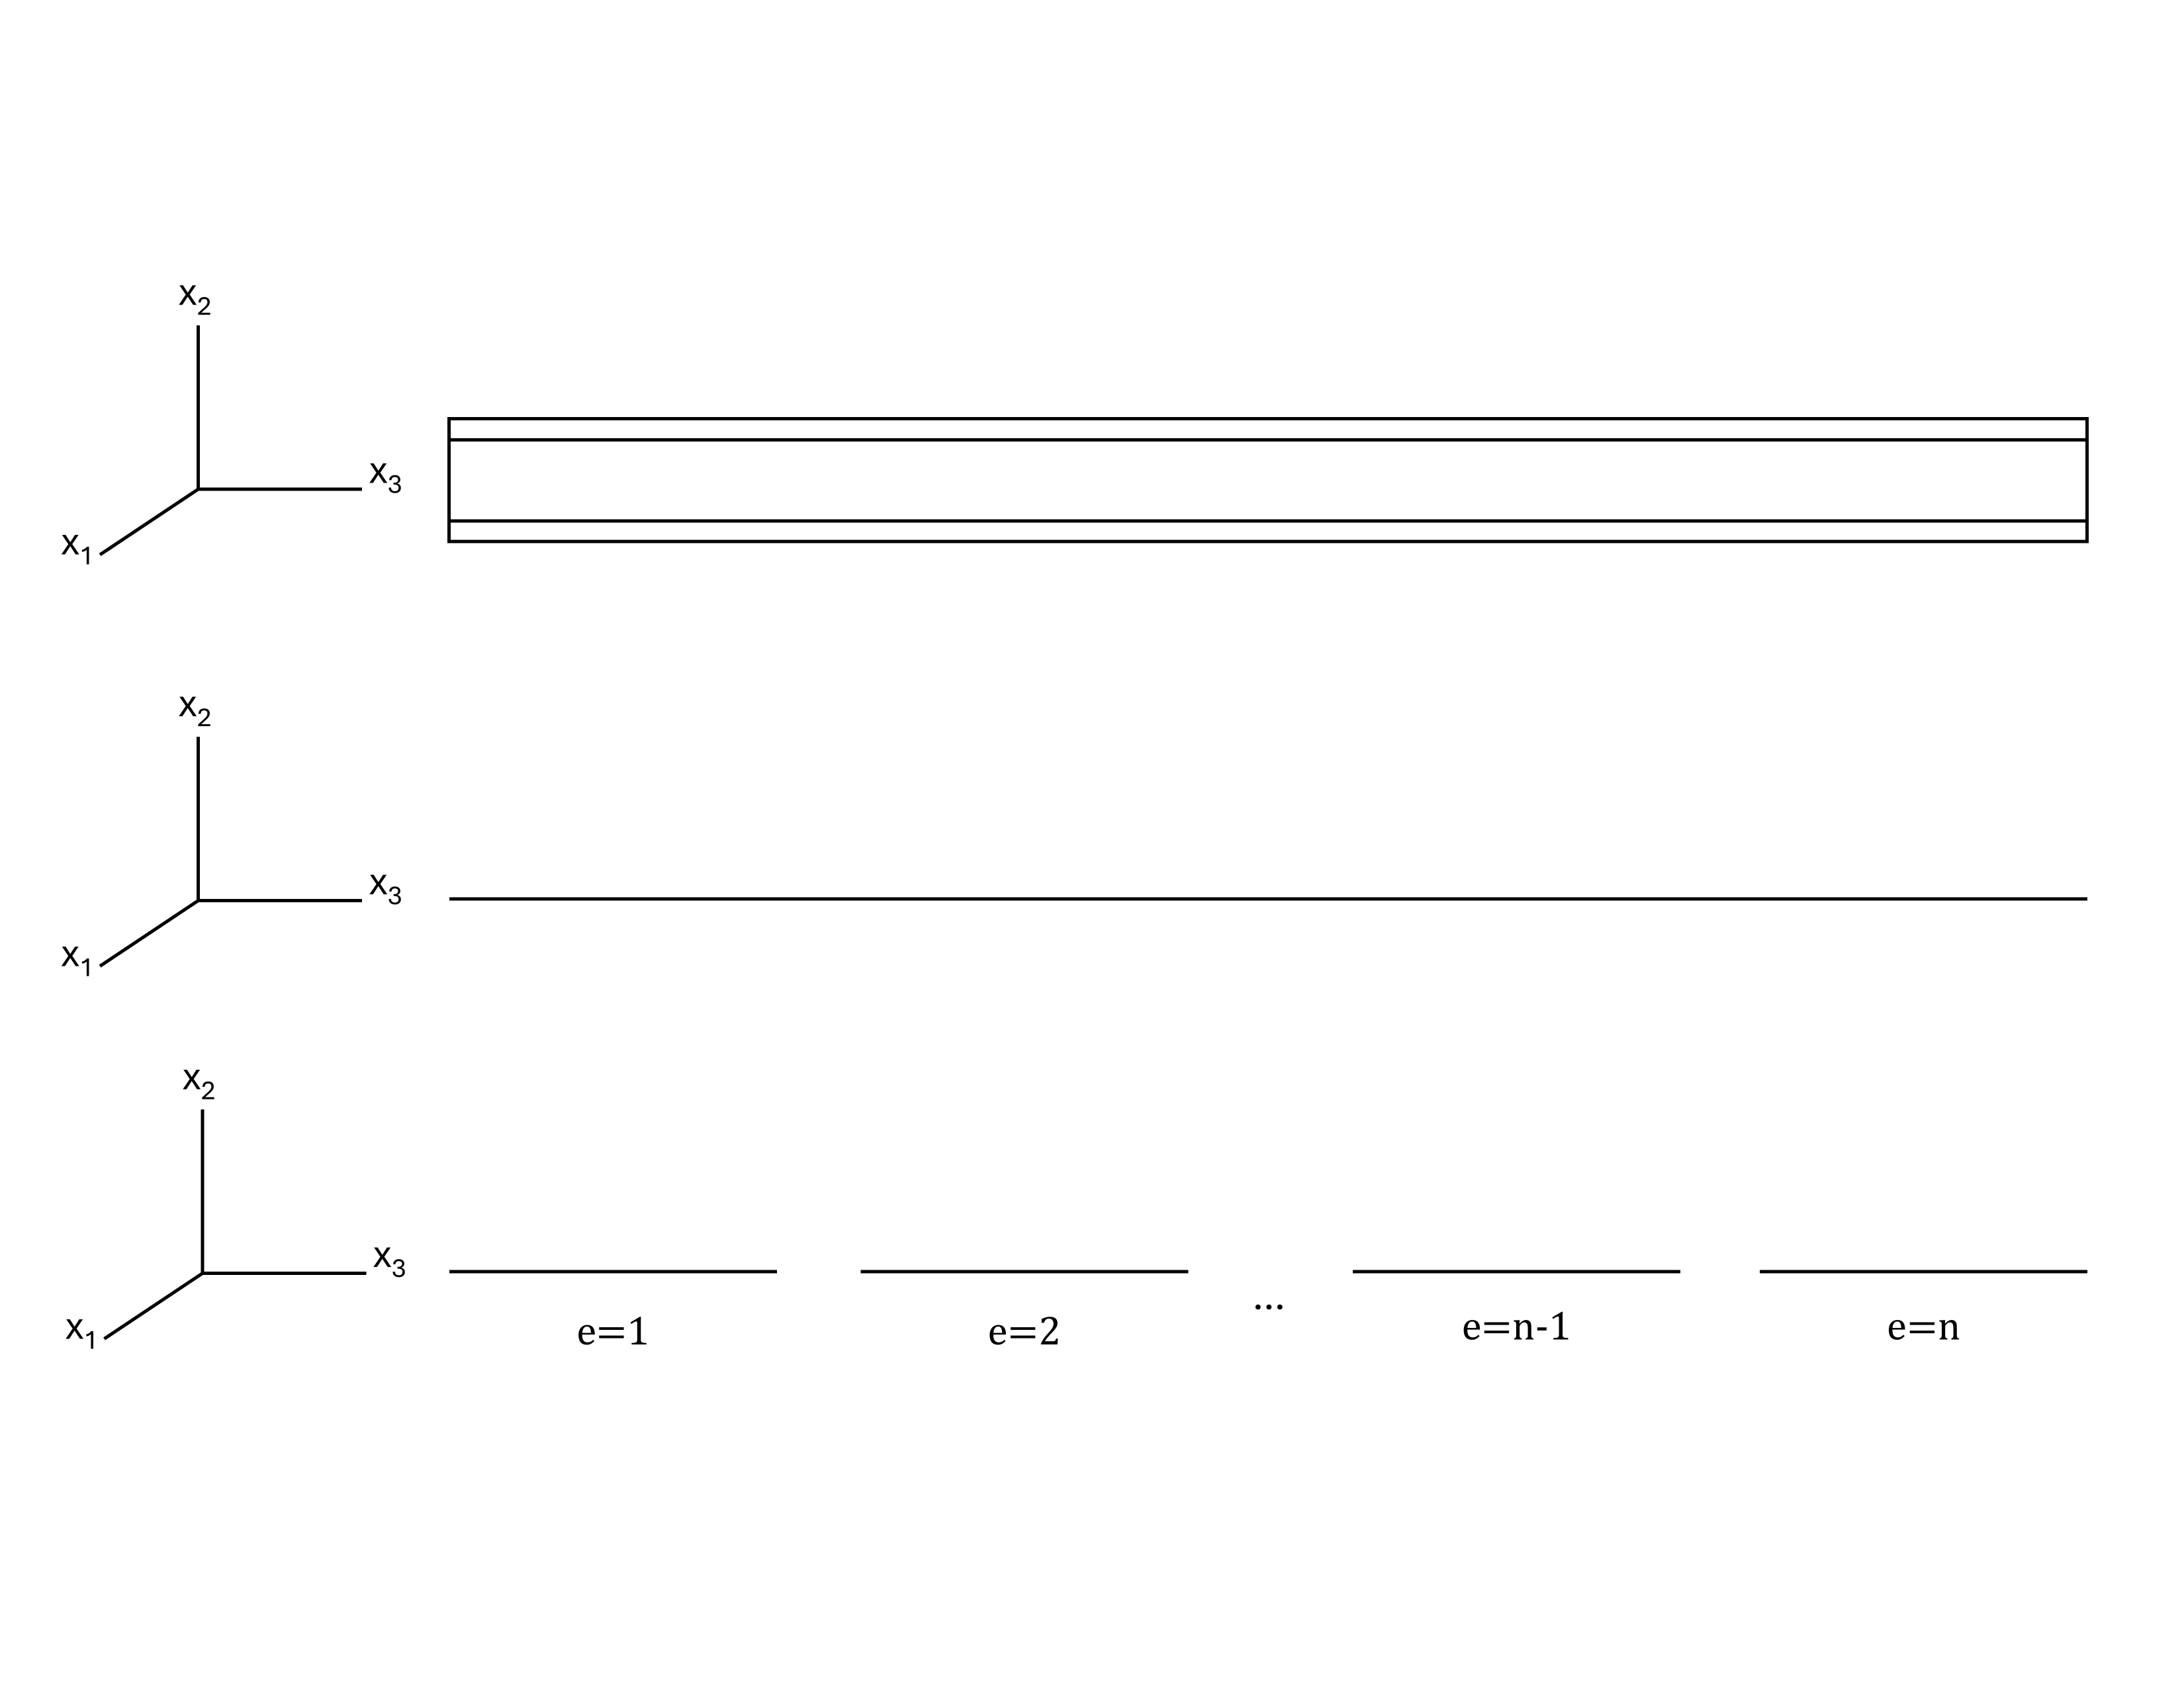
\includegraphics[width=0.7\columnwidth,trim=5.25cm 13cm 0cm 0cm, clip]{figs/beam_to_elements.png}
%}
%\centering
%\subfloat[isometric view]{
%	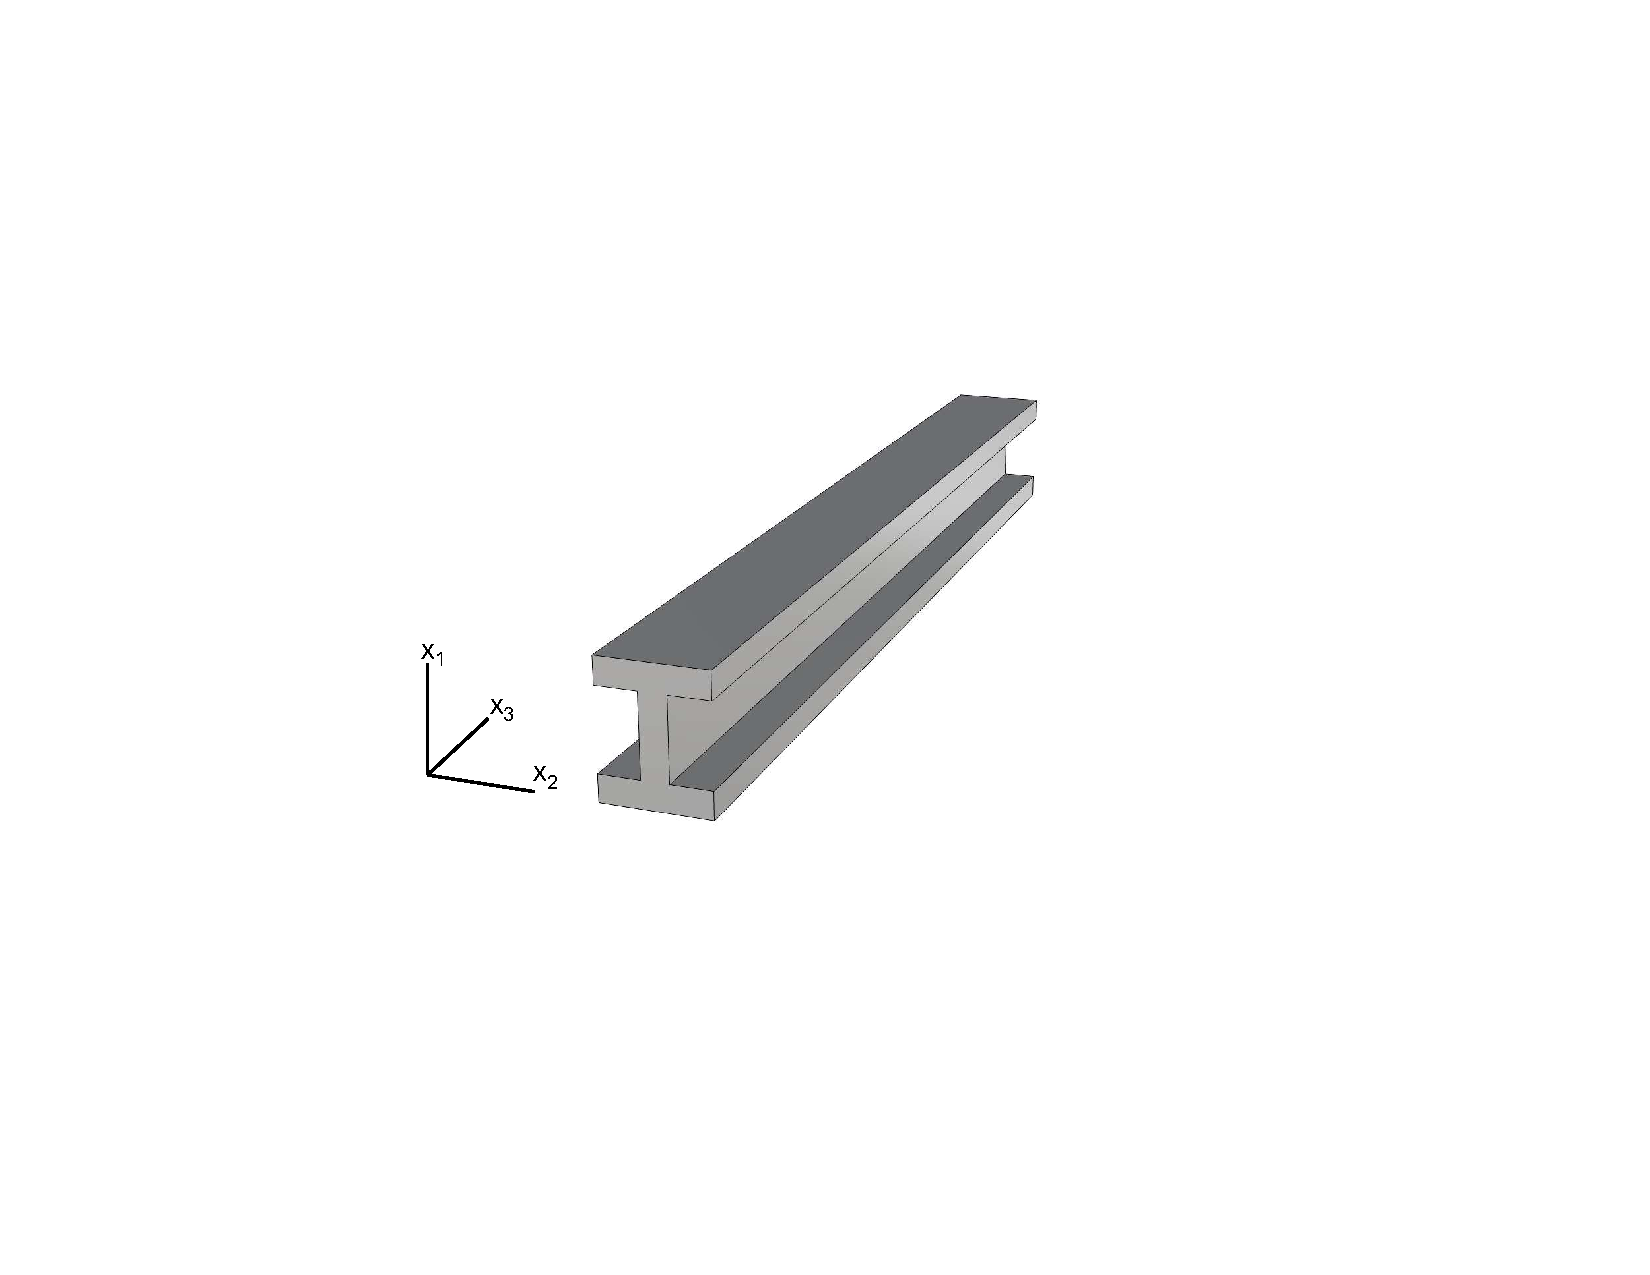
\includegraphics[width=0.25\columnwidth,trim=0cm 3cm 0cm 0cm, clip]{figs/straight.pdf}
%}
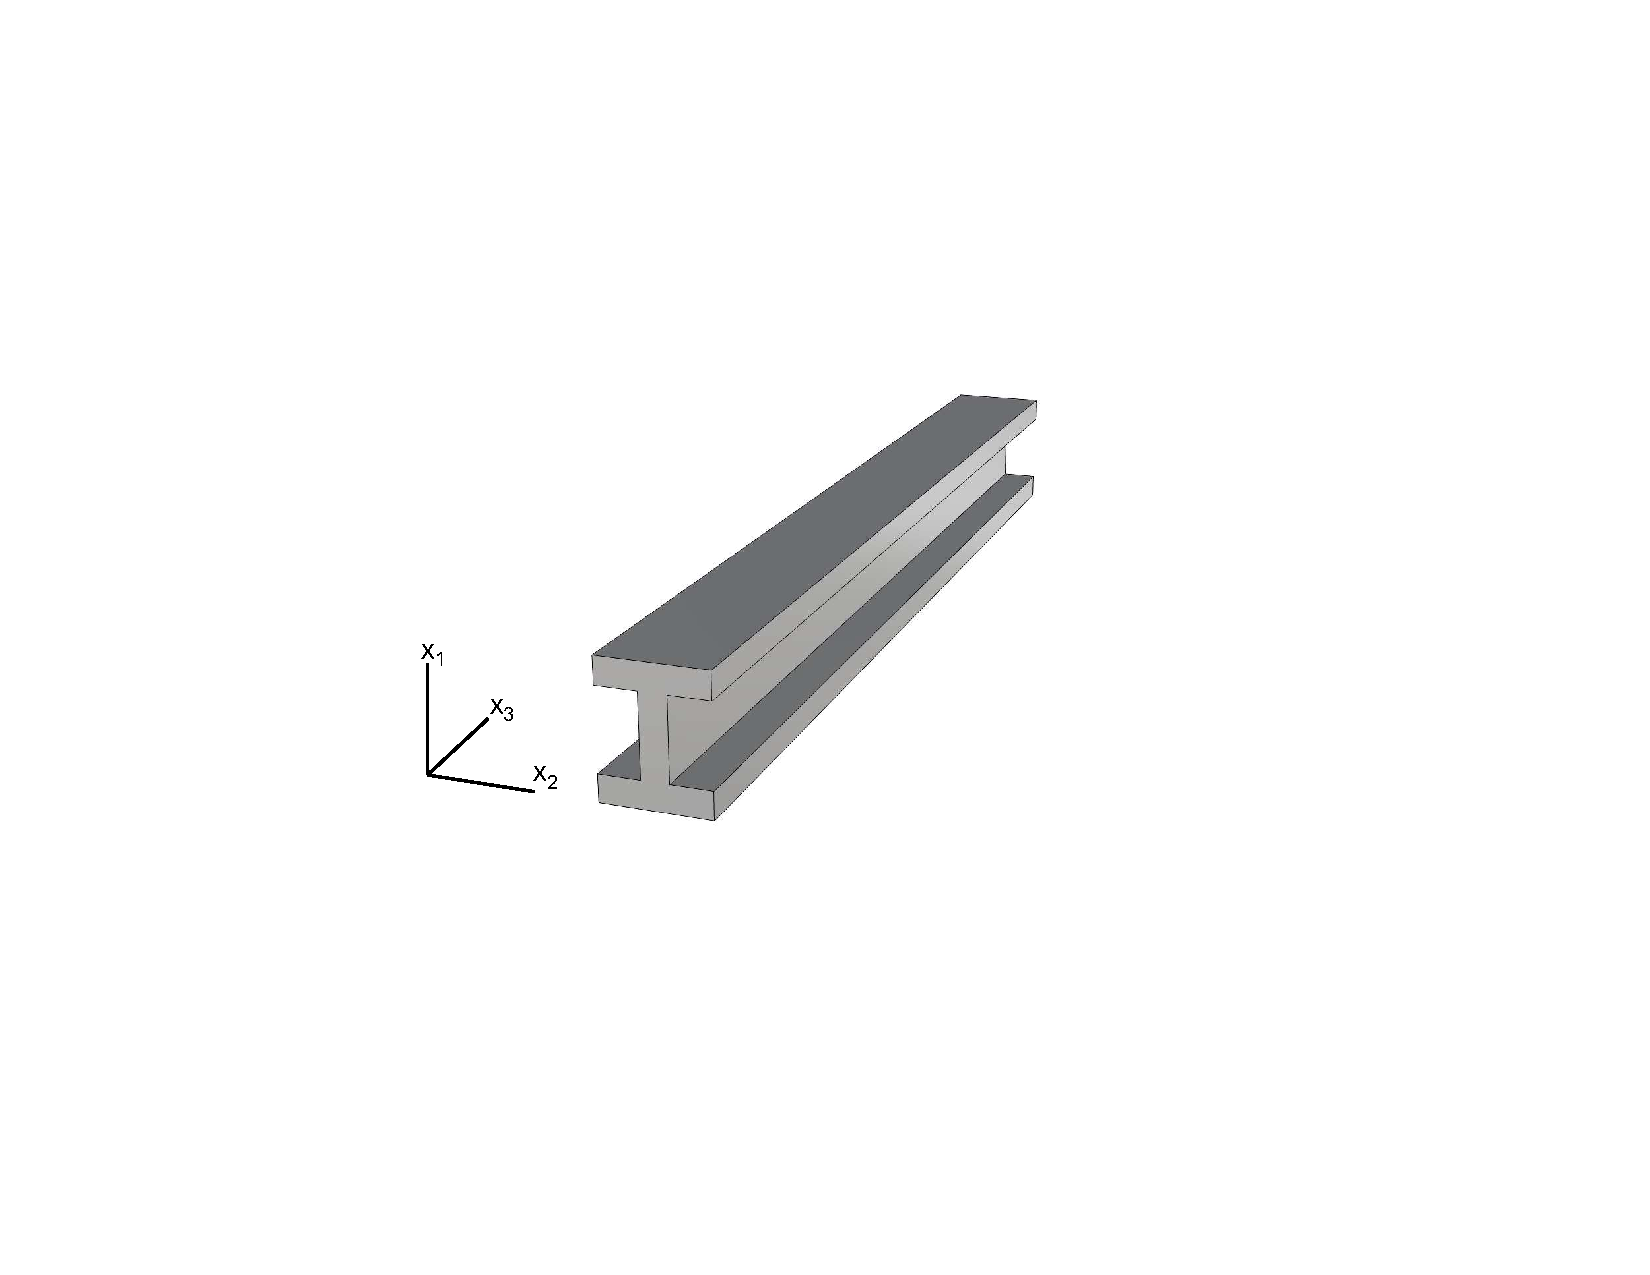
\includegraphics[width=0.95\columnwidth,trim=4cm 7cm 6cm 6.5cm, clip]{figs/straight.pdf}
\caption{The definition of the beam}
 \label{fig:beam_definition}
\end{figure}


\begin{figure}
\centering
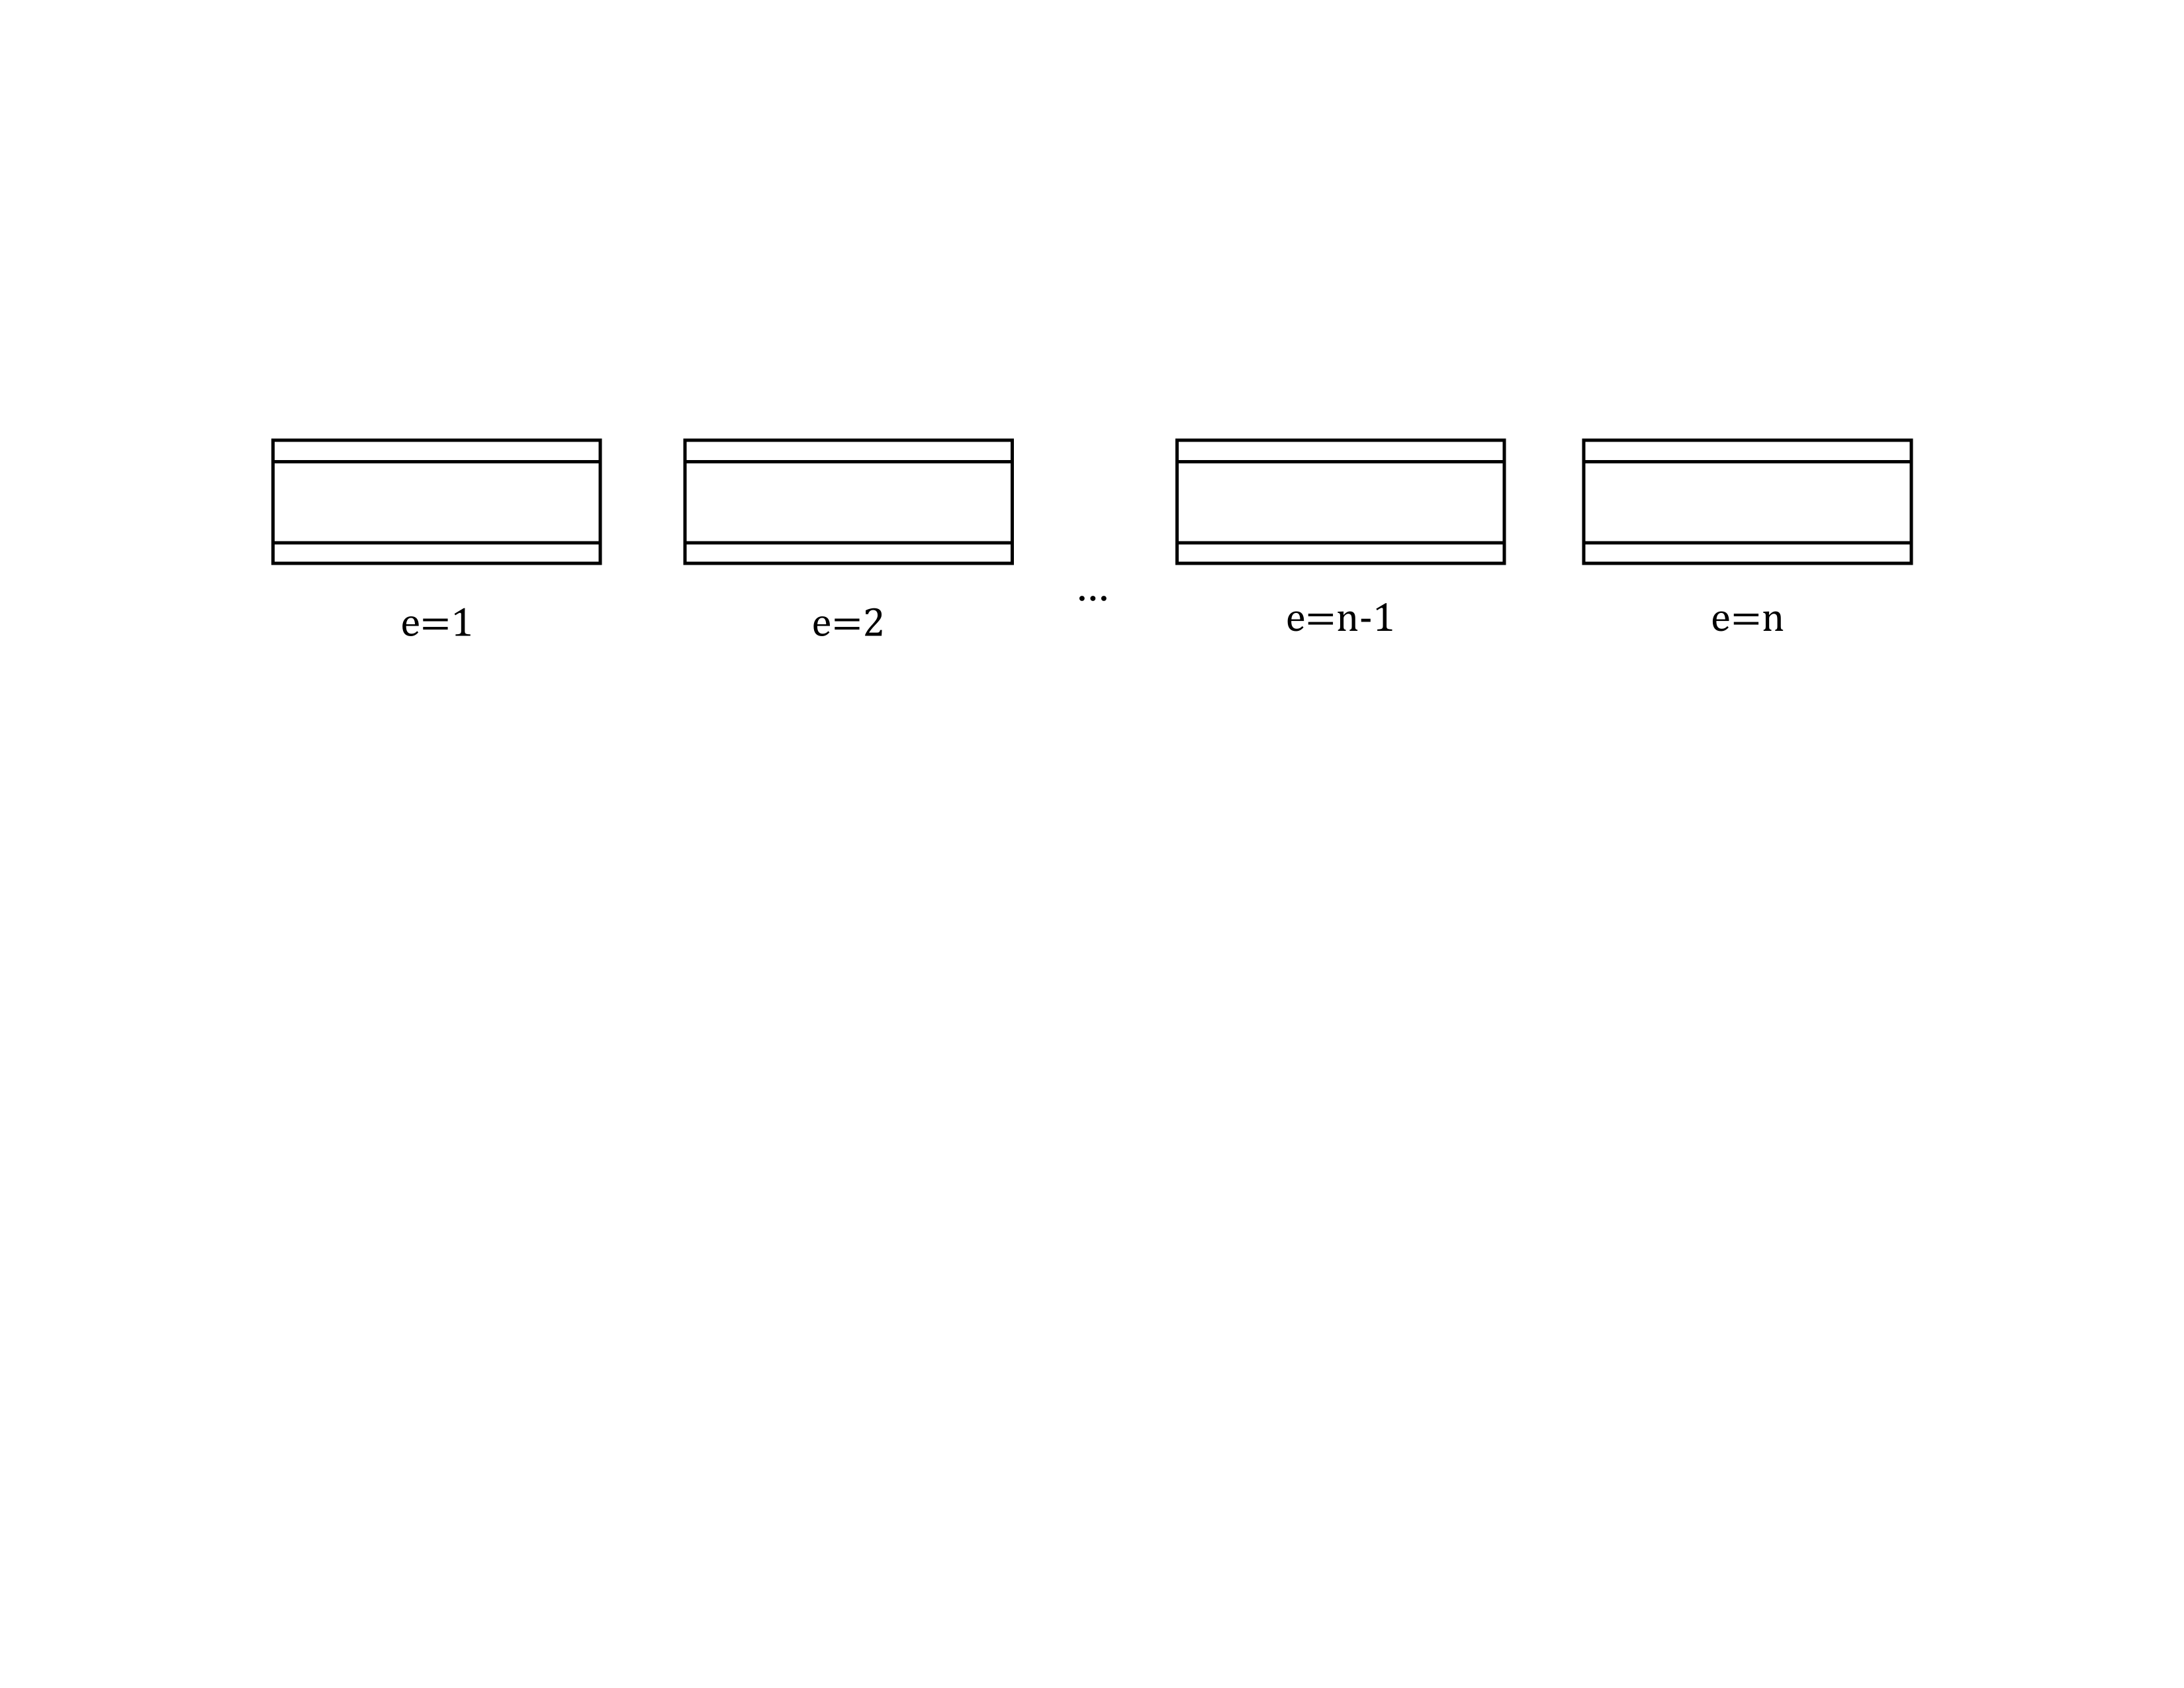
\includegraphics[width=0.7\columnwidth,trim=0cm 12cm 0cm 0cm, clip]{figs/wshape_elements.png}
\caption{The beam subdivided into n elements}
\label{fig:subdivision}
\end{figure}

\begin{figure}[htb]
\centering
\subfloat[side view]{
	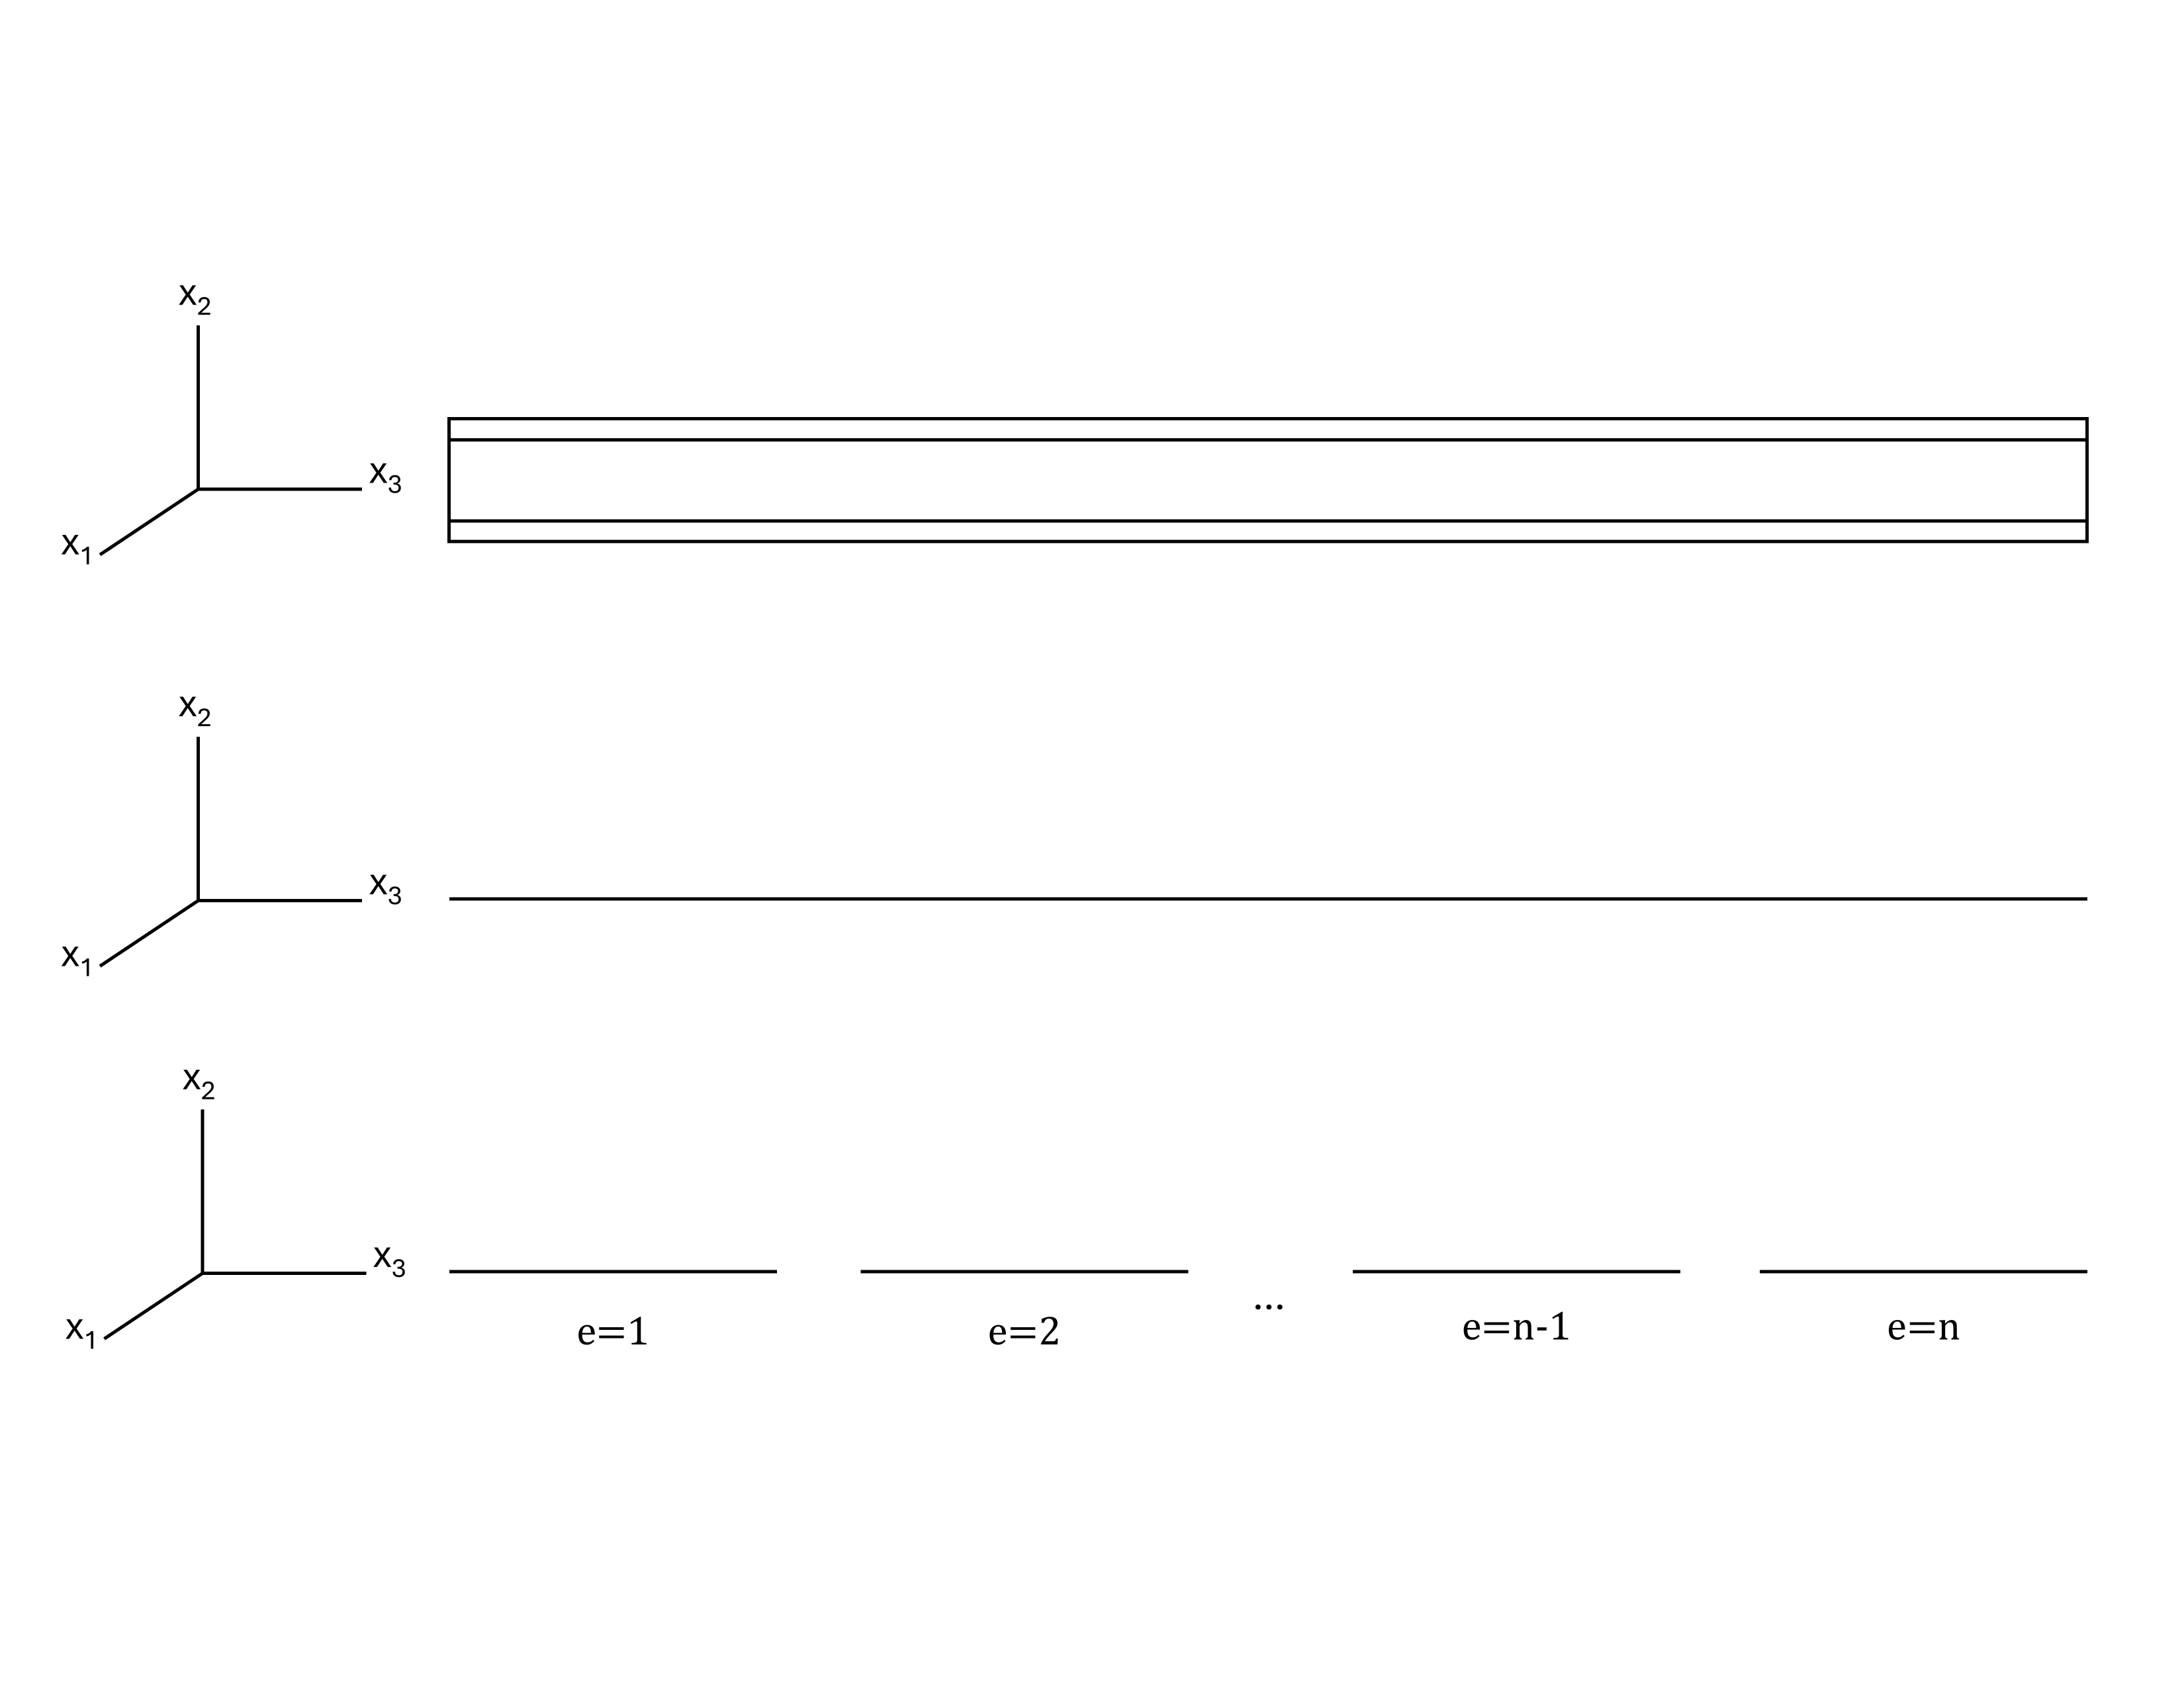
\includegraphics[width=0.7\columnwidth,trim=0cm 13cm 0cm 0cm, clip]{figs/beam_to_elements.png}
}
\centering
\subfloat[isometric view]{
	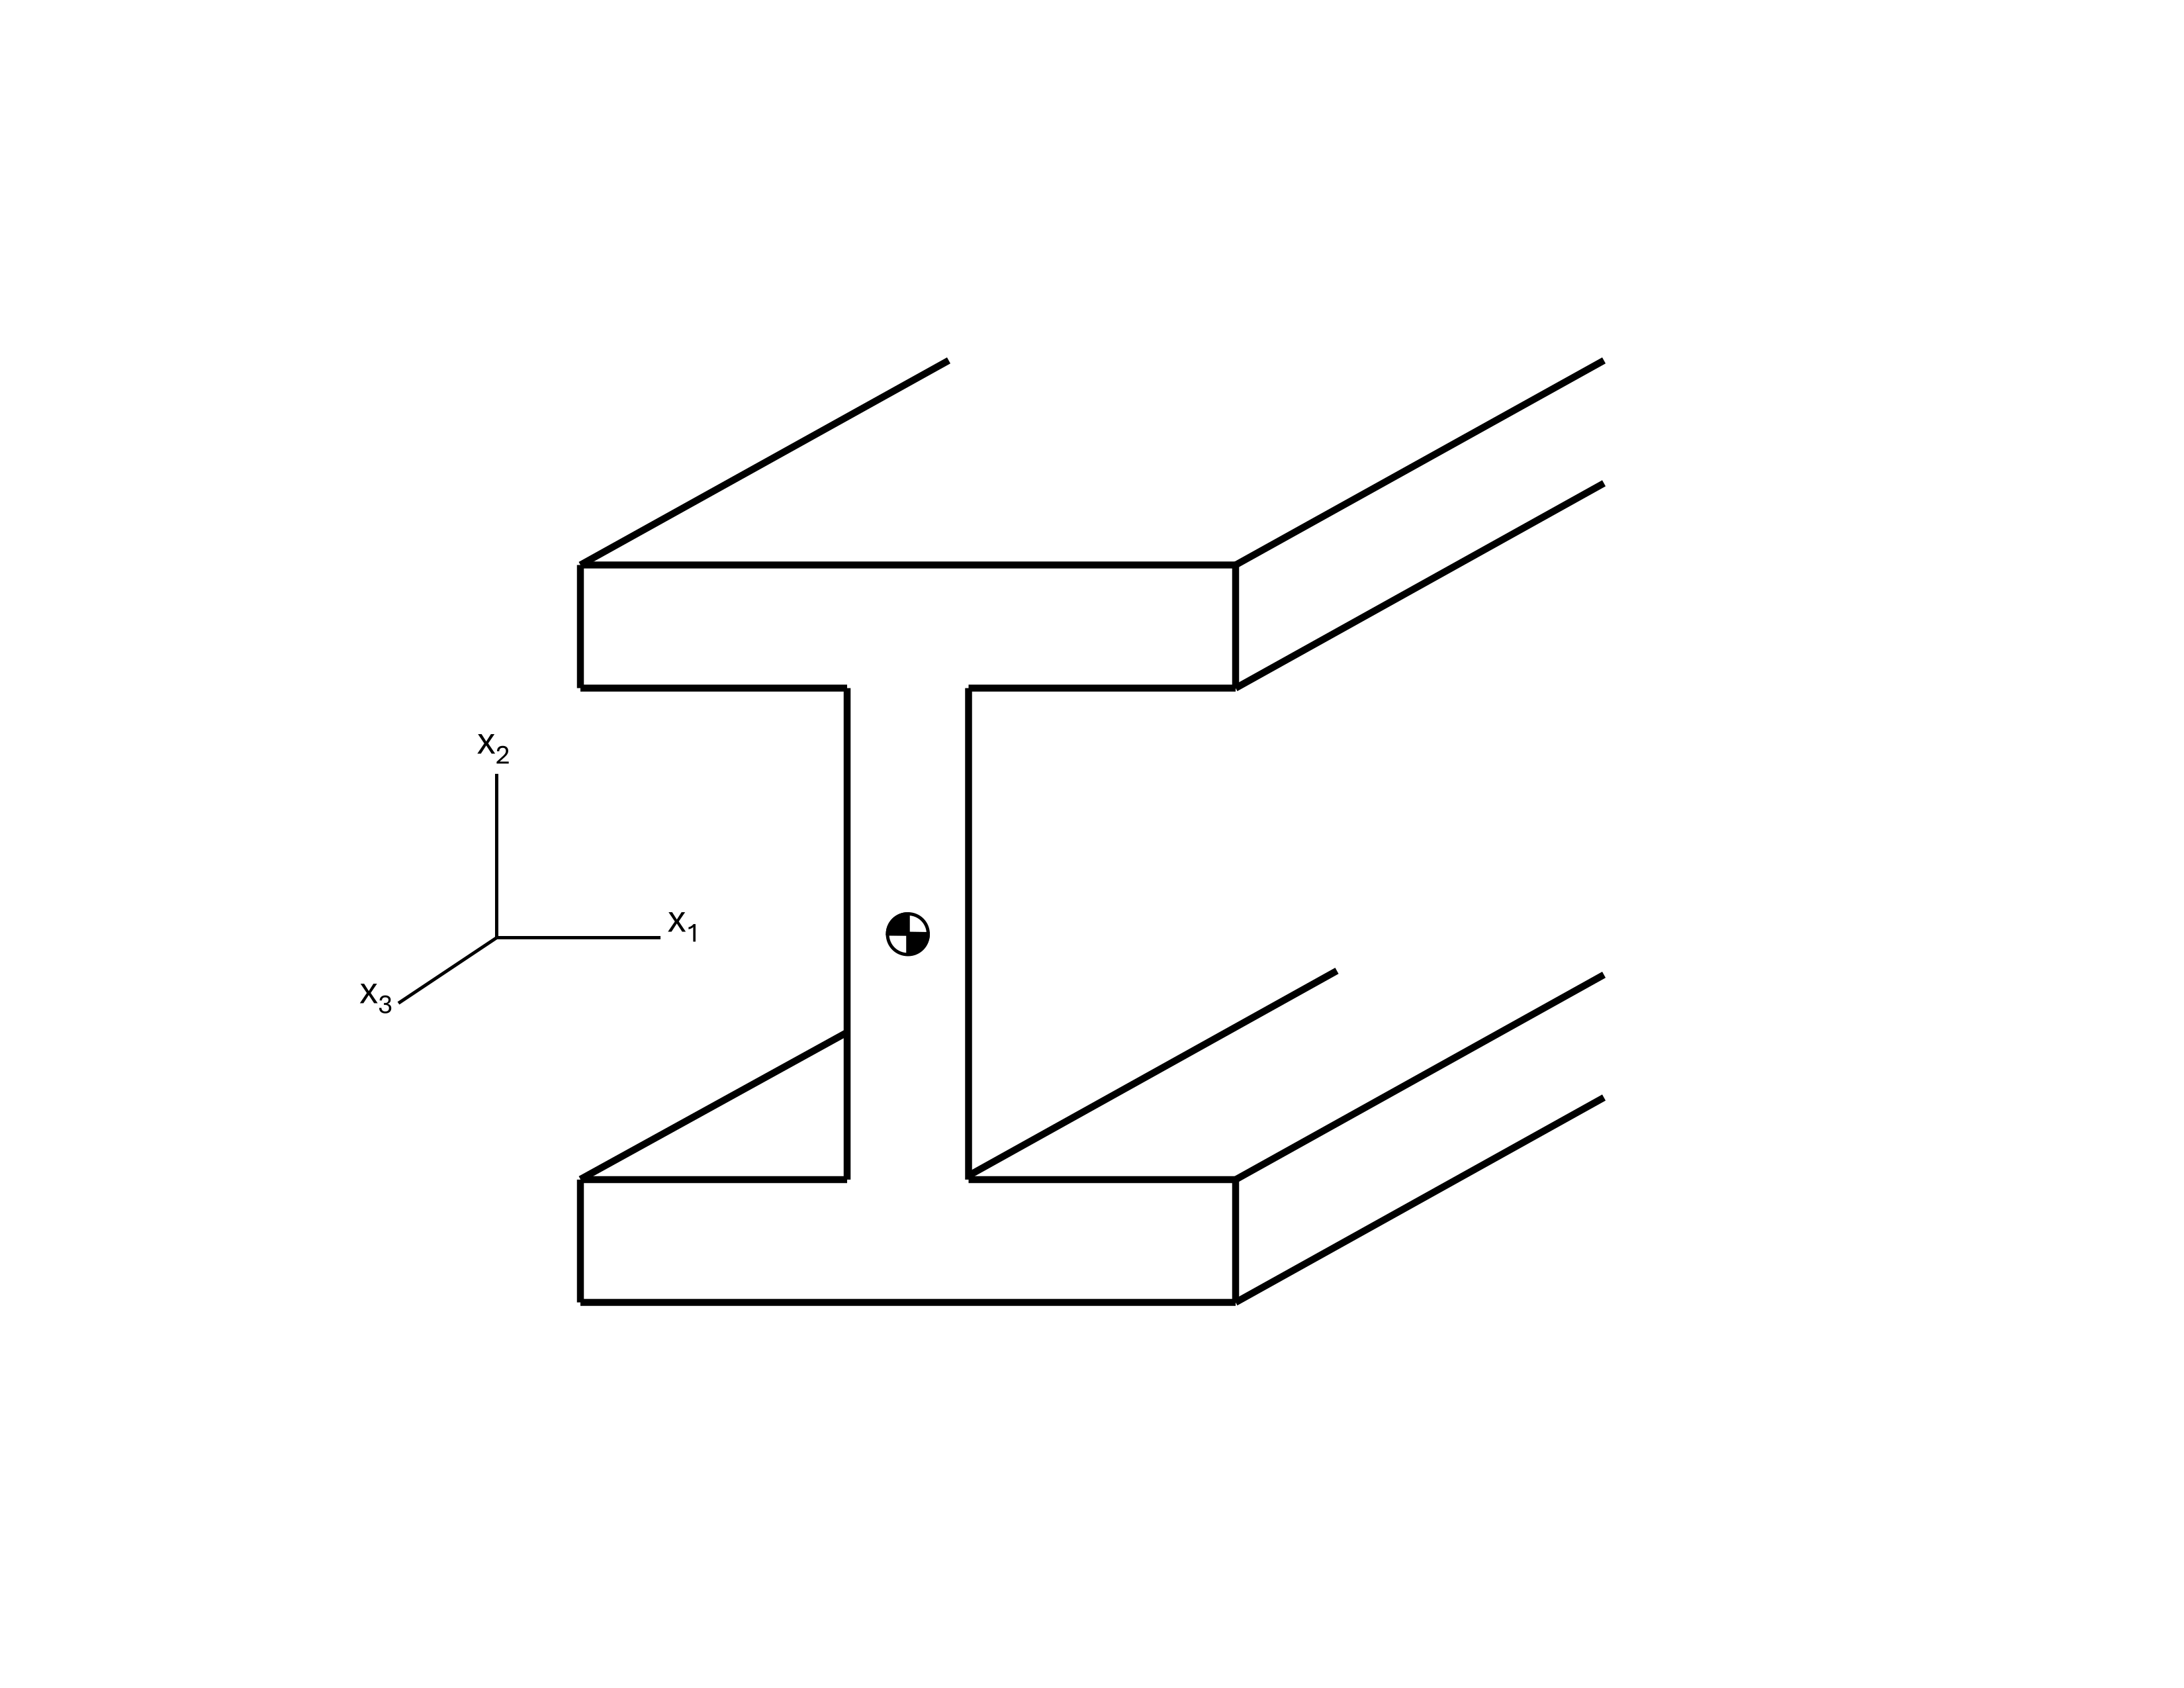
\includegraphics[width=0.25\columnwidth,trim=0cm 3cm 0cm 0cm, clip]{figs/3d_section.png}
	\label{fig:iso_view}
}
\caption{The definition of the beam}
 \label{fig:axis_definition}
\end{figure}

%I will begin by outlining the assumptions made.

\subsection{Approximating the Beam}
First a beam is defined as the domain of interest.
The beam is displayed in \cref{fig:beam_definition}.
The domain of the beam is to first be divided into multiple sections, as shown in \cref{eq:subdivision} and \cref{fig:subdivision}, where 
$\Omega$ is the beam,
$\Omega^e$  is the $e$th element of the beam, and
$\overset{n}{\underset{e=1}{\cup}}$ is the union from element 1 to n.

\begin{equation}
 \Omega = \overset{n}{\underset{e=1}{\cup}} \Omega^e
 \label{eq:subdivision}
 \end{equation}

Thus \cref{eq:subdivision} states that the domain of interest is to be composed of beam elements numbered from 1 to n.
Furthermore, each element has local axes defined with respect to the principal axes as shown in \cref{eq:axis_definition,fig:axis_definition}, where $h^e$ is the length of each element and $A^e$ is the cross sectional area of each element.

\begin{equation}
\Omega^e = \{
(x_1^e, x_2^e, x_3^e)
|x_3^e 
\in 
[0,h^e], 
(x_1^e, x_2^2) 
\in
A^e 
\subset
\mathbb{R}^2 
\}
\label{eq:axis_definition}
\end{equation}

Furthermore, for the analysis the beam will be considered a one dimensional element. 
Thus, the beam will be approximated as a line with length $h$ that will act at the centroid of the beam as shown by the center of gravity marker in~\cref{fig:iso_view}.
In other texts, this is represented by~\cref{eq:zero_area}.

\begin{equation}
0 =
\int_{A^e} x_1^e \,dA \  =
\int_{A^e} x_2^e \,dA \ =
\int_{A^e} x_1^e x_2^e \,dA \
\label{eq:zero_area}
\end{equation}




\subsection{Stress Tensor}
\label{subsec:stress_tensor}
The second assummption is that $\sigma_{\alpha\beta}=0$.
The stress tensor $\sigma$ is shown in \cref{eq:stress_tensor} and the stress element in \cref{fig:stress_element}.
%By this assumption, the beam will not have normal stresses in the $x_1$ or $x_2$ directions, similar to an axial rod.
%The difference between the beam and an axial rod is that it can experience shear in the $\sigma_{13}$ and $\sigma_{23}$ directions.
%We know the beam will have loads applied in the $x_1$ or $x_2$ directions, which typically would mean a normal stress in those directions.
%However, given our assumptions the beam will still be able to support these loads by the shear and axial force.

\begin{equation}
\sigma = \begin{bmatrix}
0 & 0 & \sigma_{13} \\
0 & 0 & \sigma_{23} \\
\sigma_{13} & \sigma_{23} & \sigma_{33}
\end{bmatrix}
\label{eq:stress_tensor}
\end{equation}

\begin{figure}%[htb]
\centering
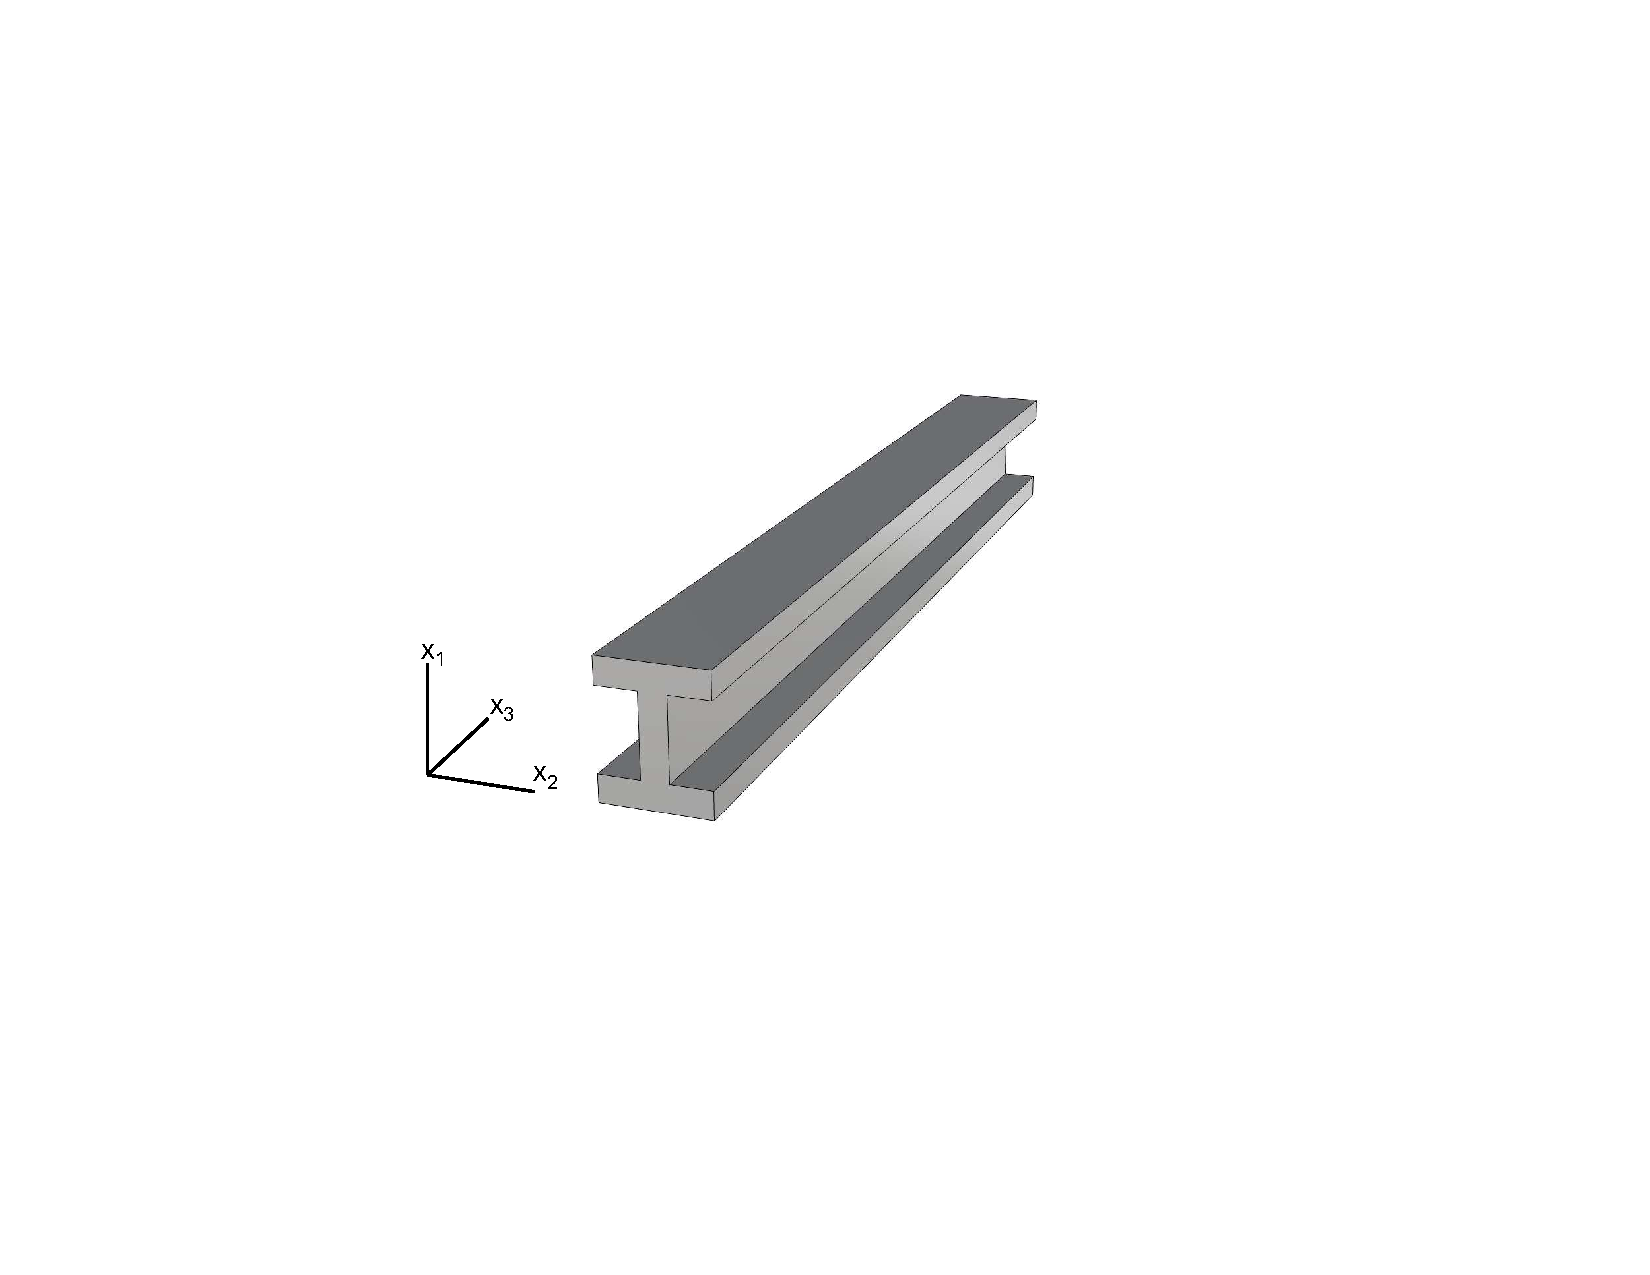
\includegraphics[width=0.95\columnwidth,trim=4cm 7cm 6cm 6.5cm, clip]{figs/straight.pdf}
\caption{The stress element of the beam in its global coordinates. CHANGE PICTURE: make a stress element with coordinate axes shown.}
\label{fig:stress_element}
\end{figure}

If we transform $\sigma$ into its principal stress form we get \cref{eq:plane_stress_tensor}.
This is significant becasue it shows that the beam is in a plane stress condition. 
A general Mohr's circle for this state of stress is shown in \cref{fig:mohrs_circle}.
This seems to justify the fact that in previous classes almost all the stress tensors we worked with were simplified to the plane stress condition or similar. 

\begin{equation}
\sigma* = \begin{bmatrix}
 \frac{\sigma_{33} + \sqrt{\sigma_{33}^2 + 4(\sigma_{13}^2 + \sigma_{23}^2)}}{2} & 0 & 0 \\
0 &  \frac{\sigma_{33} - \sqrt{\sigma_{33}^2 + 4(\sigma_{13}^2 + \sigma_{23}^2)}}{2} & 0 \\
0 & 0 & 0
\end{bmatrix}
\label{eq:plane_stress_tensor}
\end{equation}

\begin{figure}
\centering
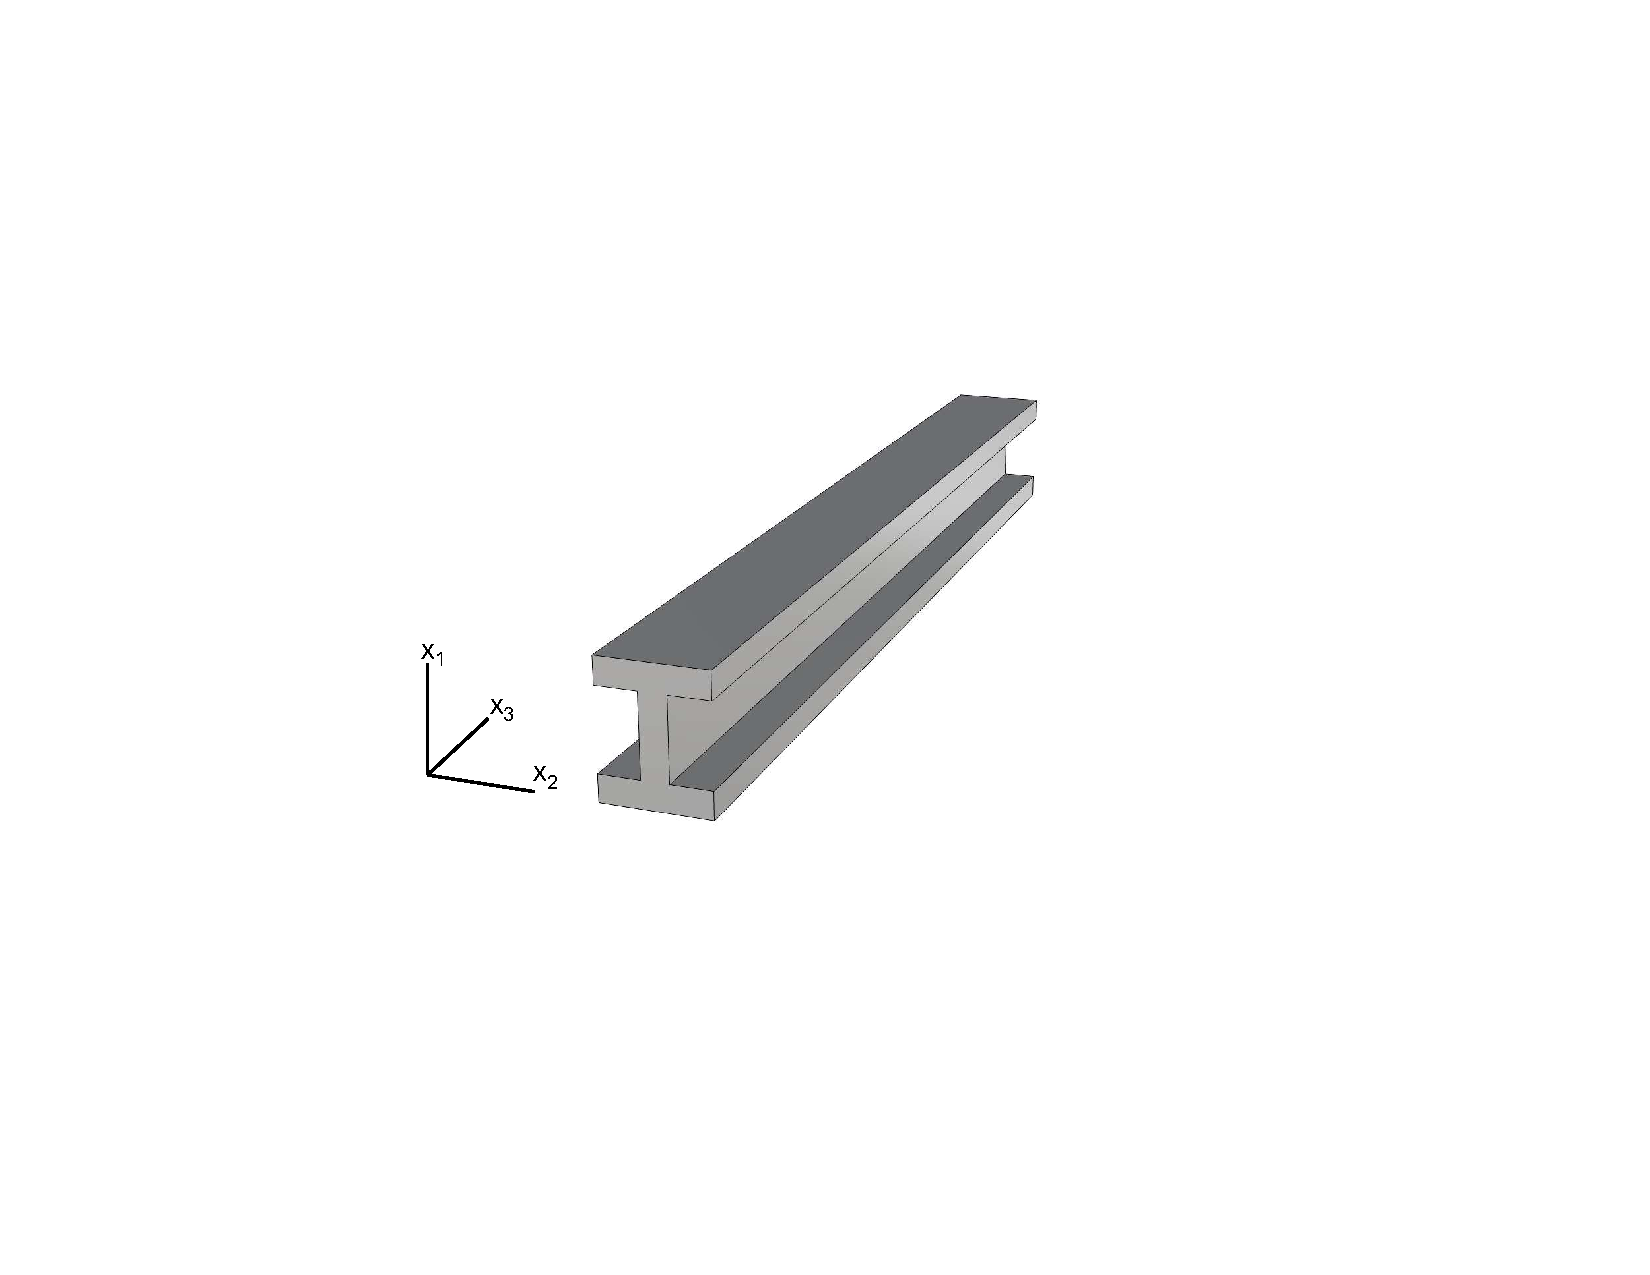
\includegraphics[width=0.95\columnwidth,trim=4cm 7cm 6cm 6.5cm, clip]{figs/straight.pdf}
\label{fig:mohrs_circle}
\caption{The generalized Mohr's circle for the plane stress condition. CHANGE PICTURE: make a Mohr's circle like the one on pg 85 (pg 25 of 61-80) in Continuum Mechanics Text}
\end{figure}

%{\Rd INCLUDE:
%This is valid by two approaches.
%
%(1) The poisson's ratio of a 1D beam must be equal to zero, because a compressive force in $x_3$ will not change the cross-section in the $x_1$ and $x_2$ directions.
%
%(2) The normal forces within the beam will be much smaller than the shear at the boundary. 
%Thus a local stress element may have normal forces ($\sigma_{11}$ and $\sigma_{22}$), but they will be much smaller than the shear at the boundary or the axial force from the moment.
%}

This assumption is less intuitive and familiar than the other assumptions made in this section.
For this reason, two approaches will be put forth to verify it's validity.
The first approach relies heavily on the one-dimensionality of the approximated beam coupled with the material properties.
The second apporach considers the details of how forces are supported using of Timoshenko Beam theory. 



\paragraph{Approach 1}
To begin, let $\epsilon_{\alpha\beta} = 0$, which is verified by \cref{eq:eps_alpha_beta_zero}.
Now, \cref{eq:stress_equations} can be derived from \cref{eq:special_hookes}.
Note that $\sigma_{\alpha\alpha}$ are not neccesarily equal to zero as previously assumed. 

\begin{align}
\sigma_{11} &= \lambda\epsilon_{33} \nonumber \\
\sigma_{22} &= \lambda\epsilon_{33} \nonumber \\
\sigma_{33} &= (\lambda+2\mu)\epsilon_{33} \nonumber \\
\sigma_{12} &= 0 \nonumber \\
\sigma_{13} &= 2\mu\epsilon_{13} \nonumber \\
\sigma_{23} &= 2\mu\epsilon_{23}
\label{eq:stress_equations}
\end{align}

Next, consider the equations for $\lambda$ and $\mu$ with respect to modulus of elasticity ($E$) and Poisson's ratio ($\nu$), see \cref{eq:lambda,eq:mu}.
%Both are dependent on the material properties modulus of elasticity ($E$) and Poisson's ratio ($\nu$).
%For $\lambda$ to be equal to zero, either $E$ or $\nu$ must be equal to zero.
%Now consider the physical meaning of setting them to zero.
%For $E = 0$ the beam would have no stiffness.
%It would not be able to handle any loads, including selfweight.
%For $\nu = 0$ the beam would not experience a change in cross-sectional area when loaded axially.

\begin{equation}
\lambda = \frac{\nu E}{(1+\nu)(1-2\nu)}
\label{eq:lambda}
\end{equation}

\begin{equation}
\mu =  \frac{2E}{2(1+\nu)}
\label{eq:mu}
\end{equation}

The physical representation of $\nu$ deals with the compresibility of a material.
%The stiffness of the material is described by $E$. 
%A more stiff material will have a higher value of $E$ and vice versa. 
For a material in axial compression, $\nu$ represents the materials tendency to expand in the transverse direction.
The values of $\nu$ may range from 0 to 0.5.
If $\nu = 0$ the material will experience no exapnsion when compressed.
On the other hand, when $\nu = 0.5$ it will expand to maintain a constant volume. 

Although $\nu$ is a material property, it's siginificance may be influenced by geometry.
For example, an axial rod of length $l$ and diameter $d$ is composed of an isotropic material with a maximal Poisson's ration $\nu = 0.5$.
When this rod is tensioned to stretch some $\Delta l$, the diameter will also change by some $\Delta d$ so that the volume $V$ does not change.
If the rod is slender, then $\Delta d << \Delta l$.
Therefore, $\Delta d$ may be negligible for a sufficiently slender rod.

The approximated beam is the most extreme case of a slender element because it is one-dimensional.
The cross-section will not expand or contract under compression or tension. 
Therefore, $\nu$ must be equal to zero.
Consequently, $\lambda$ will also be zero.
If we substitute zero for $\lambda$ in \cref{eq:stress_equations}, we obtain that $\sigma_{\alpha\alpha} = 0$.

%Obviously, making $E$ go to zero would completely nullify the purpose of analyzing the beam.
%However, for our beam idealized as a 1D element $\nu$ must be equal to zero.
%A 1D line has no cross-sectional area, therefore there can be no bulging or narrowing of the beam.
%This assumption is valid because $\sqrt A << h$, so even though our beam will expand or contract slightly it will be negligible compared to the axial deformation. 
%{\Rd change this to go from the 1D beam to meet at $\nu = 0$ rather than exploring both $E$ and $\nu$ equal to zero}.
%
%Therefore, because $\nu = 0$ then $\lambda=0$ also and thus $sigma_{\alpha \beta} = 0$.


\paragraph{Approach 2}
%For the beam under consideration, the stresses will vary linearly throughout the beam. 
%
%A beam is controlled by moment or shear.
%Our beam is defined to support axial force and shear.
%For the current theory moment is converted to an axial force in the analysis ($F = My/EI$), so it may also take moment.
%
%In this case, on a local scale $\sigma_{\alpha\beta} may not be zero. 
%However, on a global scale $\sigma_{\alpha\beta} << V,M$ so it is safe to approximate $\sigma_{\alpha\beta} = 0$.

The controlling internal forces of a beam are moment and shear.
By the above assumptions, the beam is capable of supporting shear and axial force.
By Timoshenko beam theory the moment is transfered into an axial force in the beam ($\sigma_{bending}=\frac{My}{I}$).
In this manner, the controlling forces are accounted for.

Locally, the beam may experience nonzero $\sigma_{\alpha\beta}$ stresses.
However, these stresses will be much smaller than the controling shear and moment-induced axial forces.
This will be to the degree that the transverse normal forces will be negligible. 
Thus, it is reasonable to make the global approximation that $\sigma_{\alpha\beta}=0$





\subsection{Kinematics}
\label{subsec:displacements}
The kinematics of the beam will be accounted for using \cref{eq:u1,eq:u2,eq:u3}.
The translation of the beam is represented by $w_i$, where $i$ is the direction of the translation.
The rotation of the beam is represented by $\theta_i$.
As can be observed from the equations, $w_i$ and $\theta_i$ are functions of only $x_3$, the location along the length of the beam.
That is true because the beam is collapsed to a one-dimensional element.
The overall displacement of a point on the beam is $u_i$, which acts as a function of $x_1$, $x_2$, and $x_3$.
\cref{fig:w_theta_displacements} displays a positive displacement in each coordinate direction for both translations and rotations. 

\begin{equation}
u_1(x_1, x_2, x_3)=w_1(x_3)-x_2\theta_3(x_3)
\label{eq:u1}
\end{equation}

\begin{equation}
u_2(x_1, x_2, x_3)=w_2(x_3)+x_1\theta_3(x_3)
\label{eq:u2}
\end{equation}

\begin{equation}
u_3(x_1, x_2, x_3)=w_3(x_3)-x_1\theta_2(x_3)+x_2\theta_1(x_3)
\label{eq:u3}
\end{equation}

\begin{figure}
\centering
\subfloat[No displacement]{
	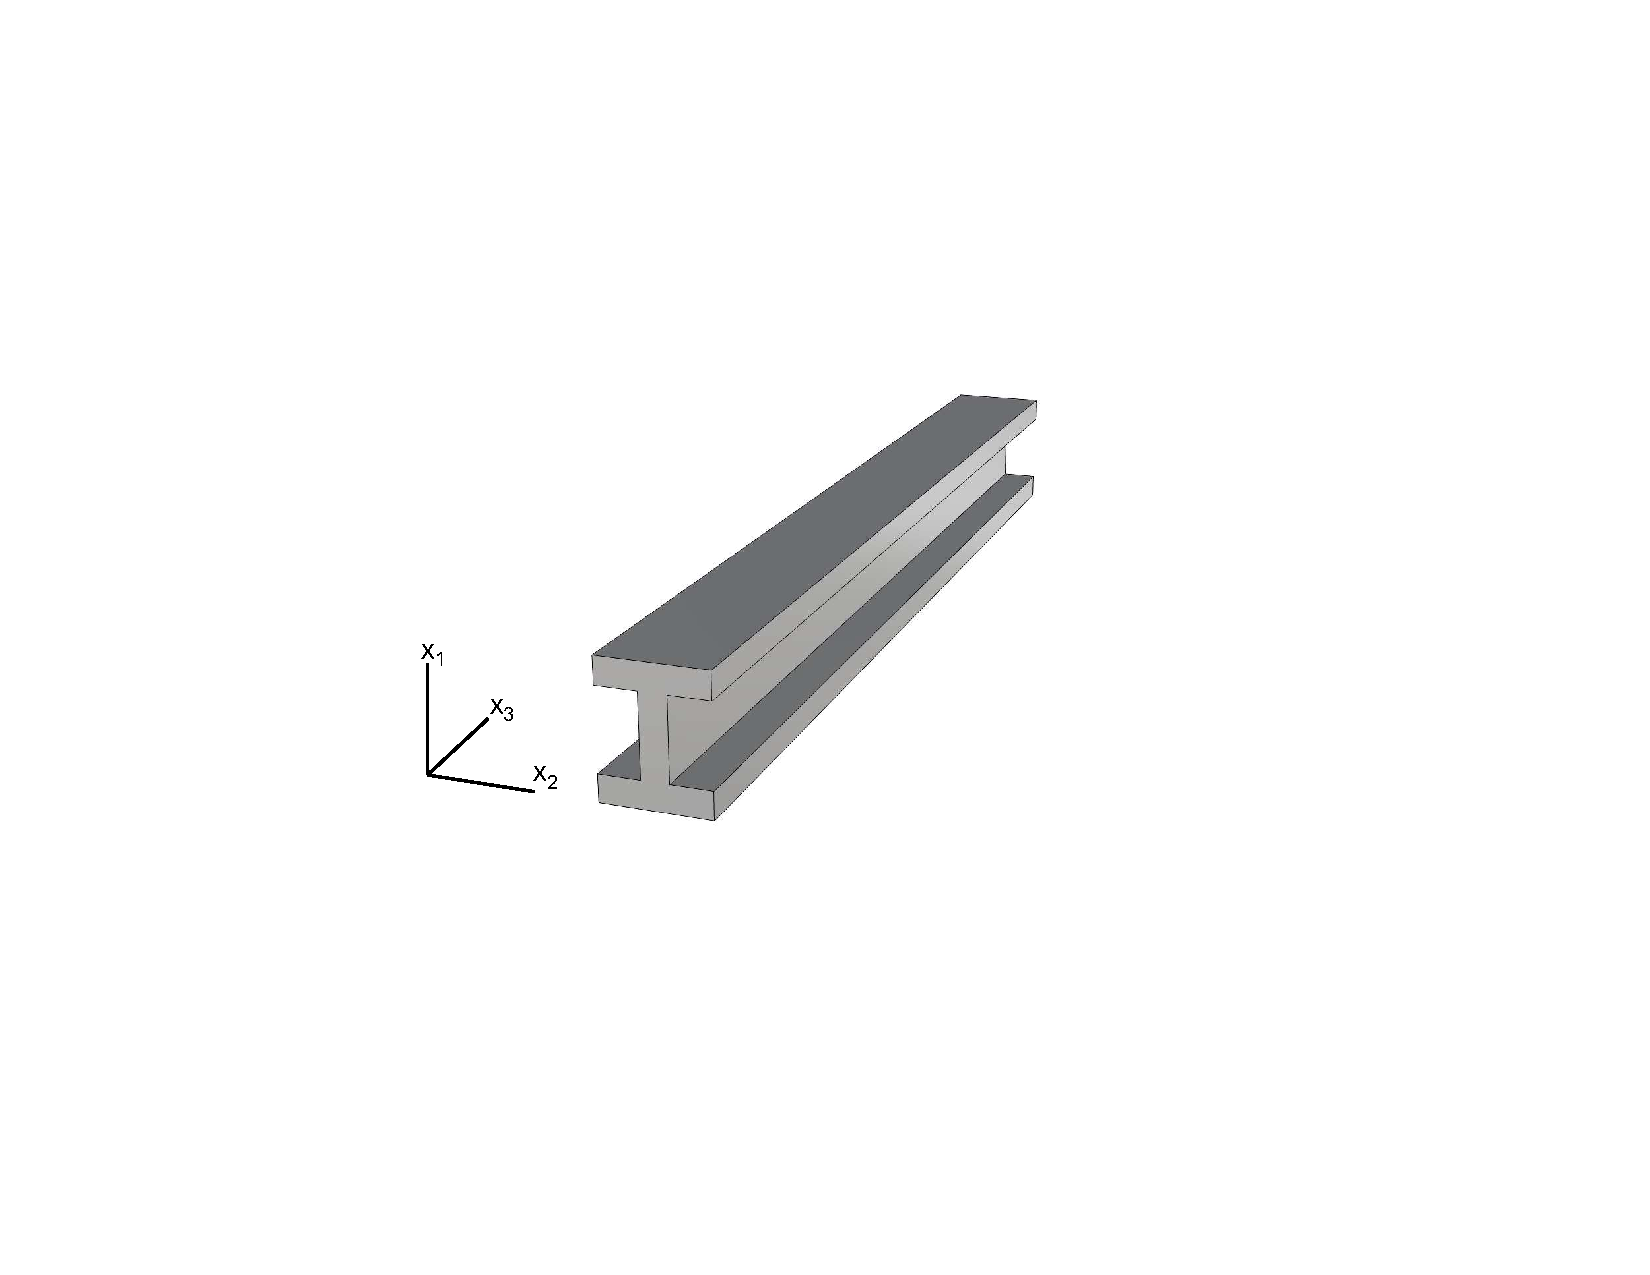
\includegraphics[width=0.2\columnwidth,trim=4cm 7cm 6cm 6.5cm, clip]{figs/straight.pdf}
}
\\
\subfloat[$w_1$]{
	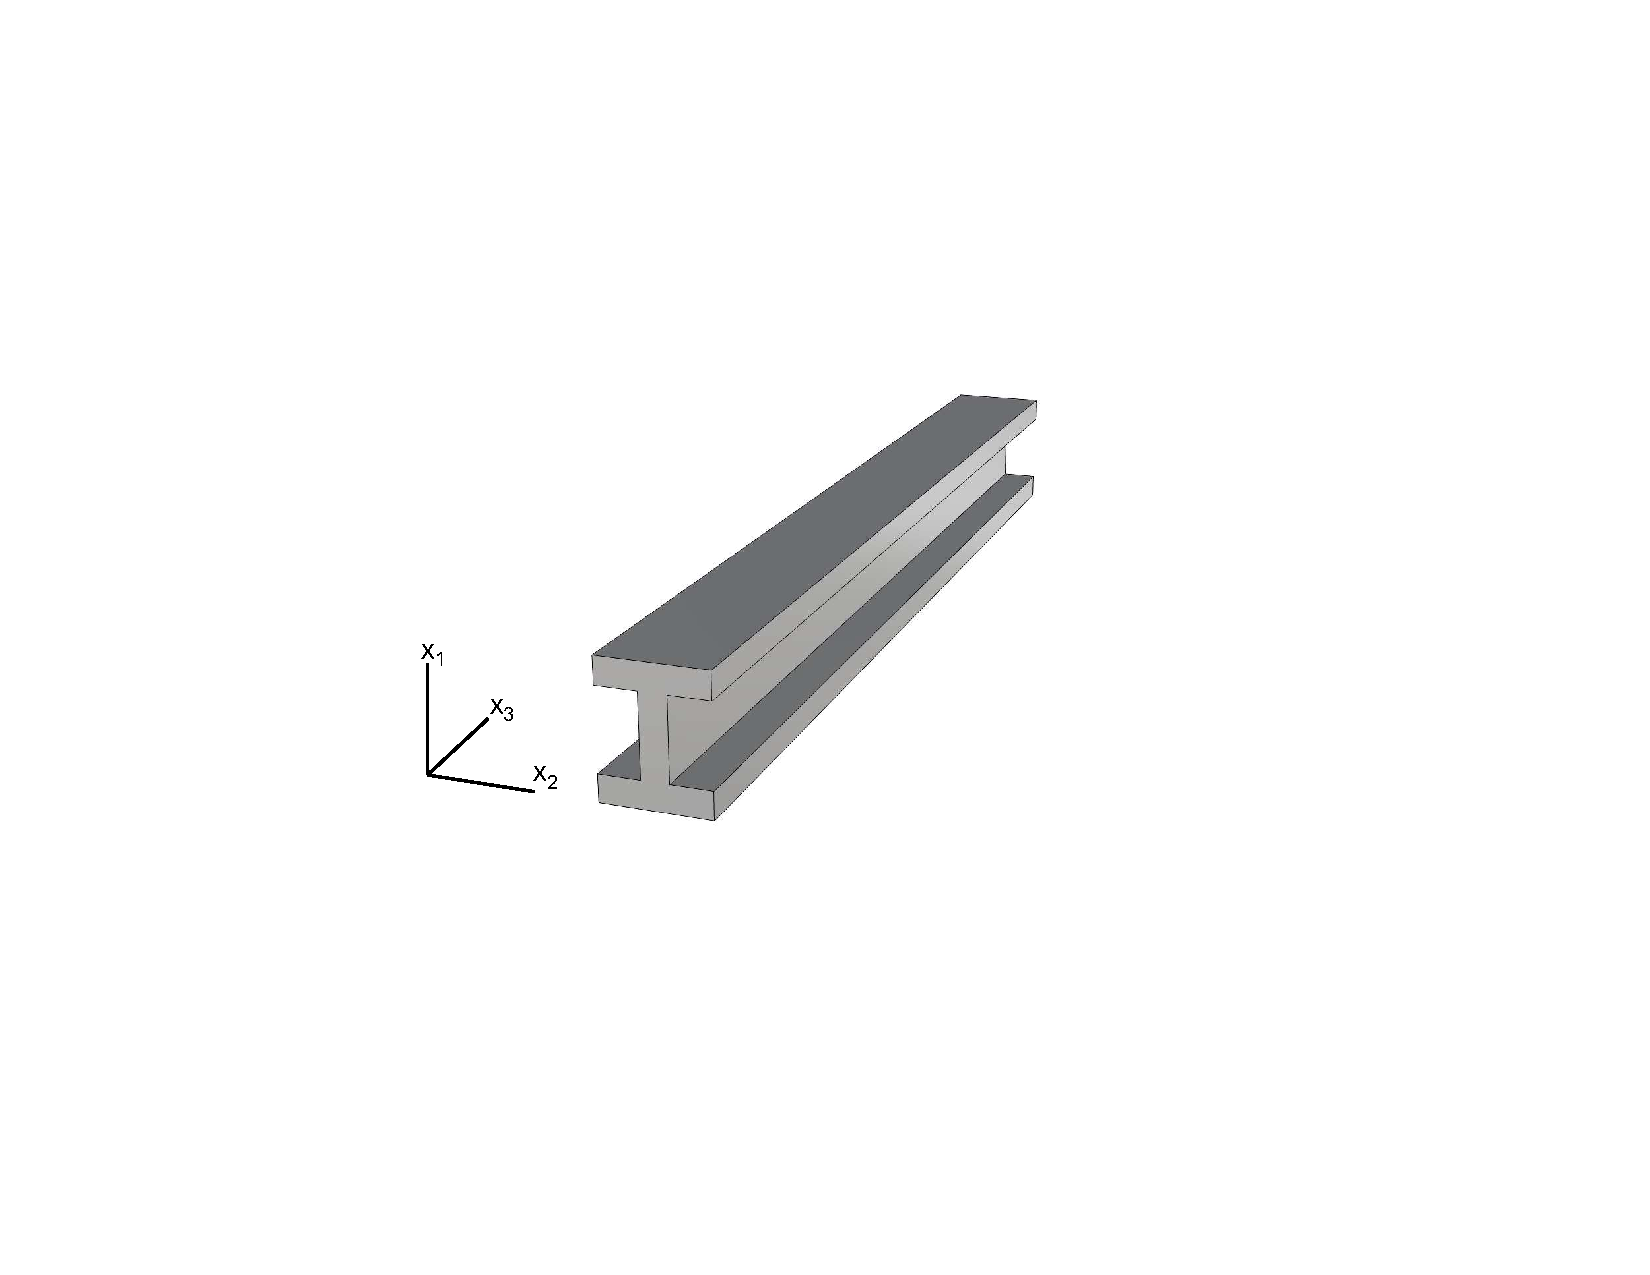
\includegraphics[width=0.2\columnwidth,trim=4cm 7cm 6cm 6.5cm, clip]{figs/straight.pdf}
}
\subfloat[$w_2$]{
	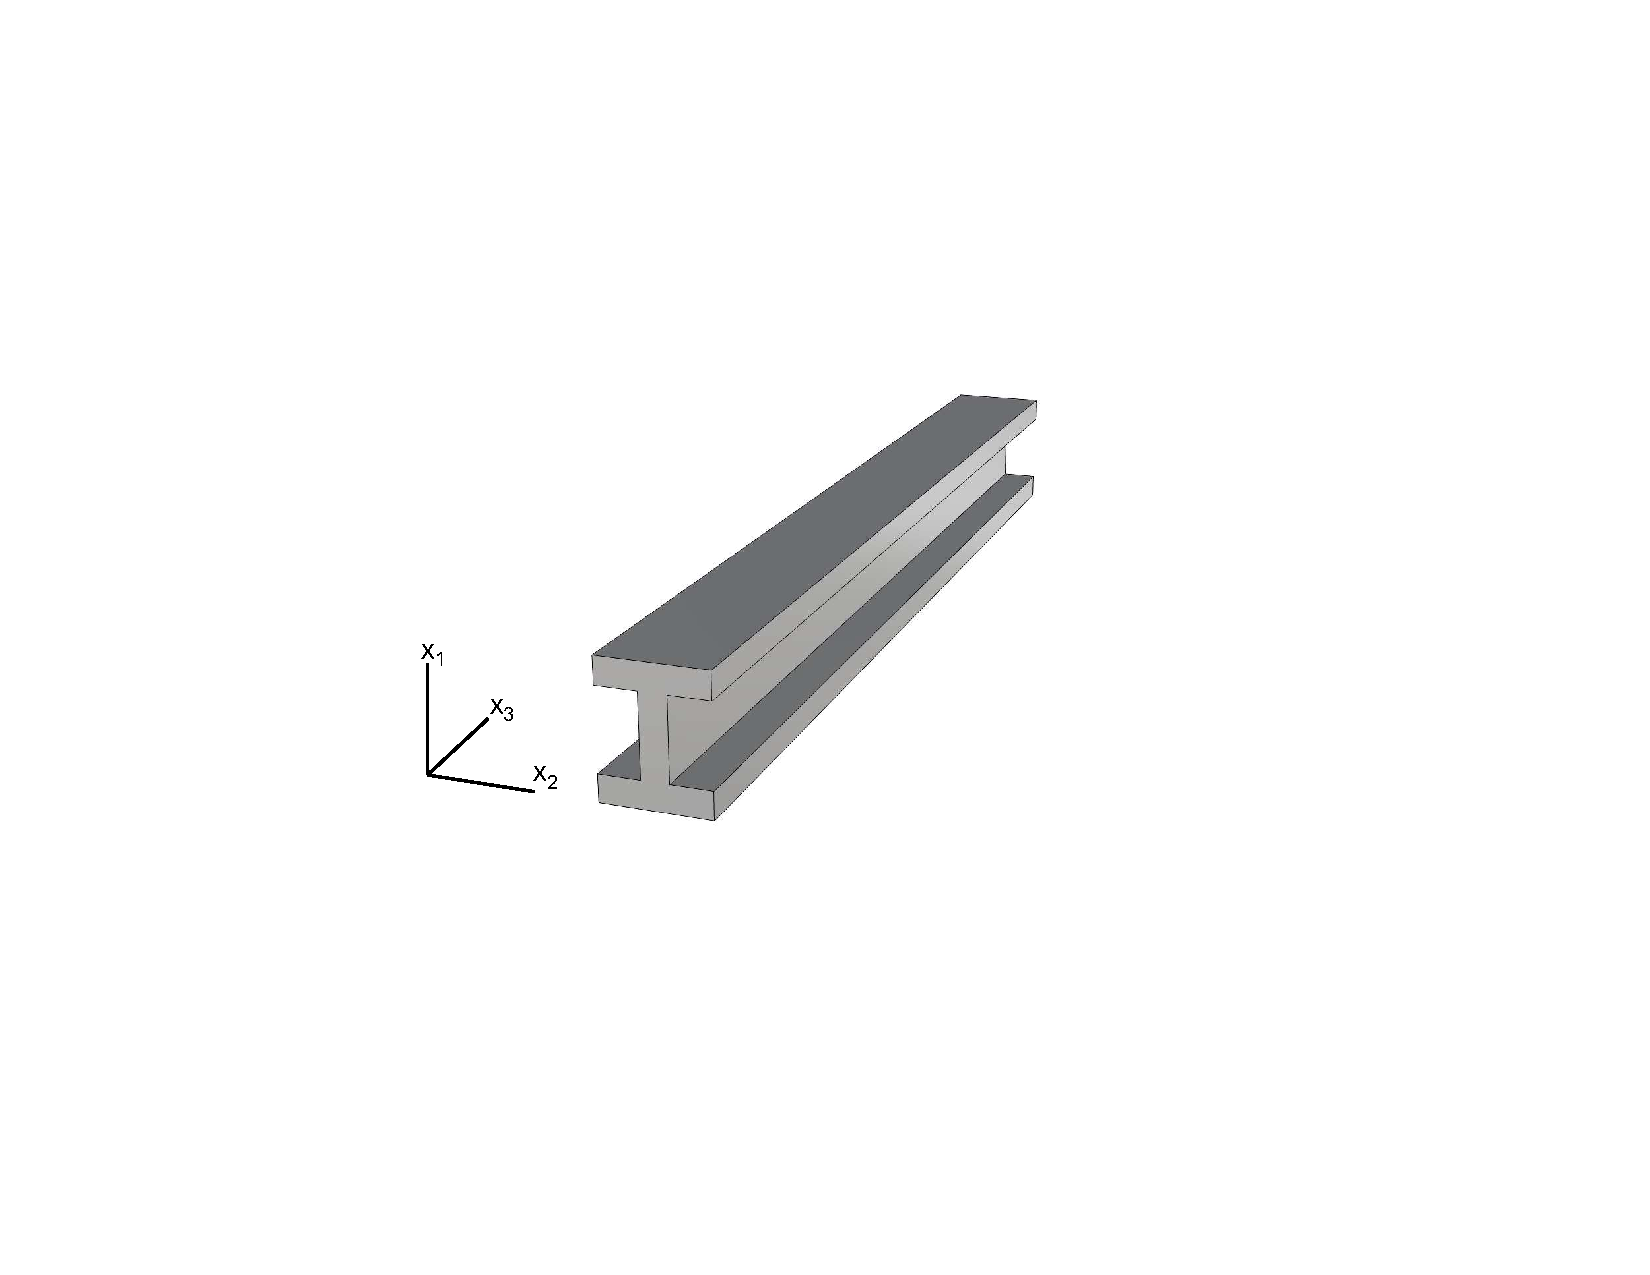
\includegraphics[width=0.2\columnwidth,trim=4cm 7cm 6cm 6.5cm, clip]{figs/straight.pdf}
}
\subfloat[$w_3$]{
	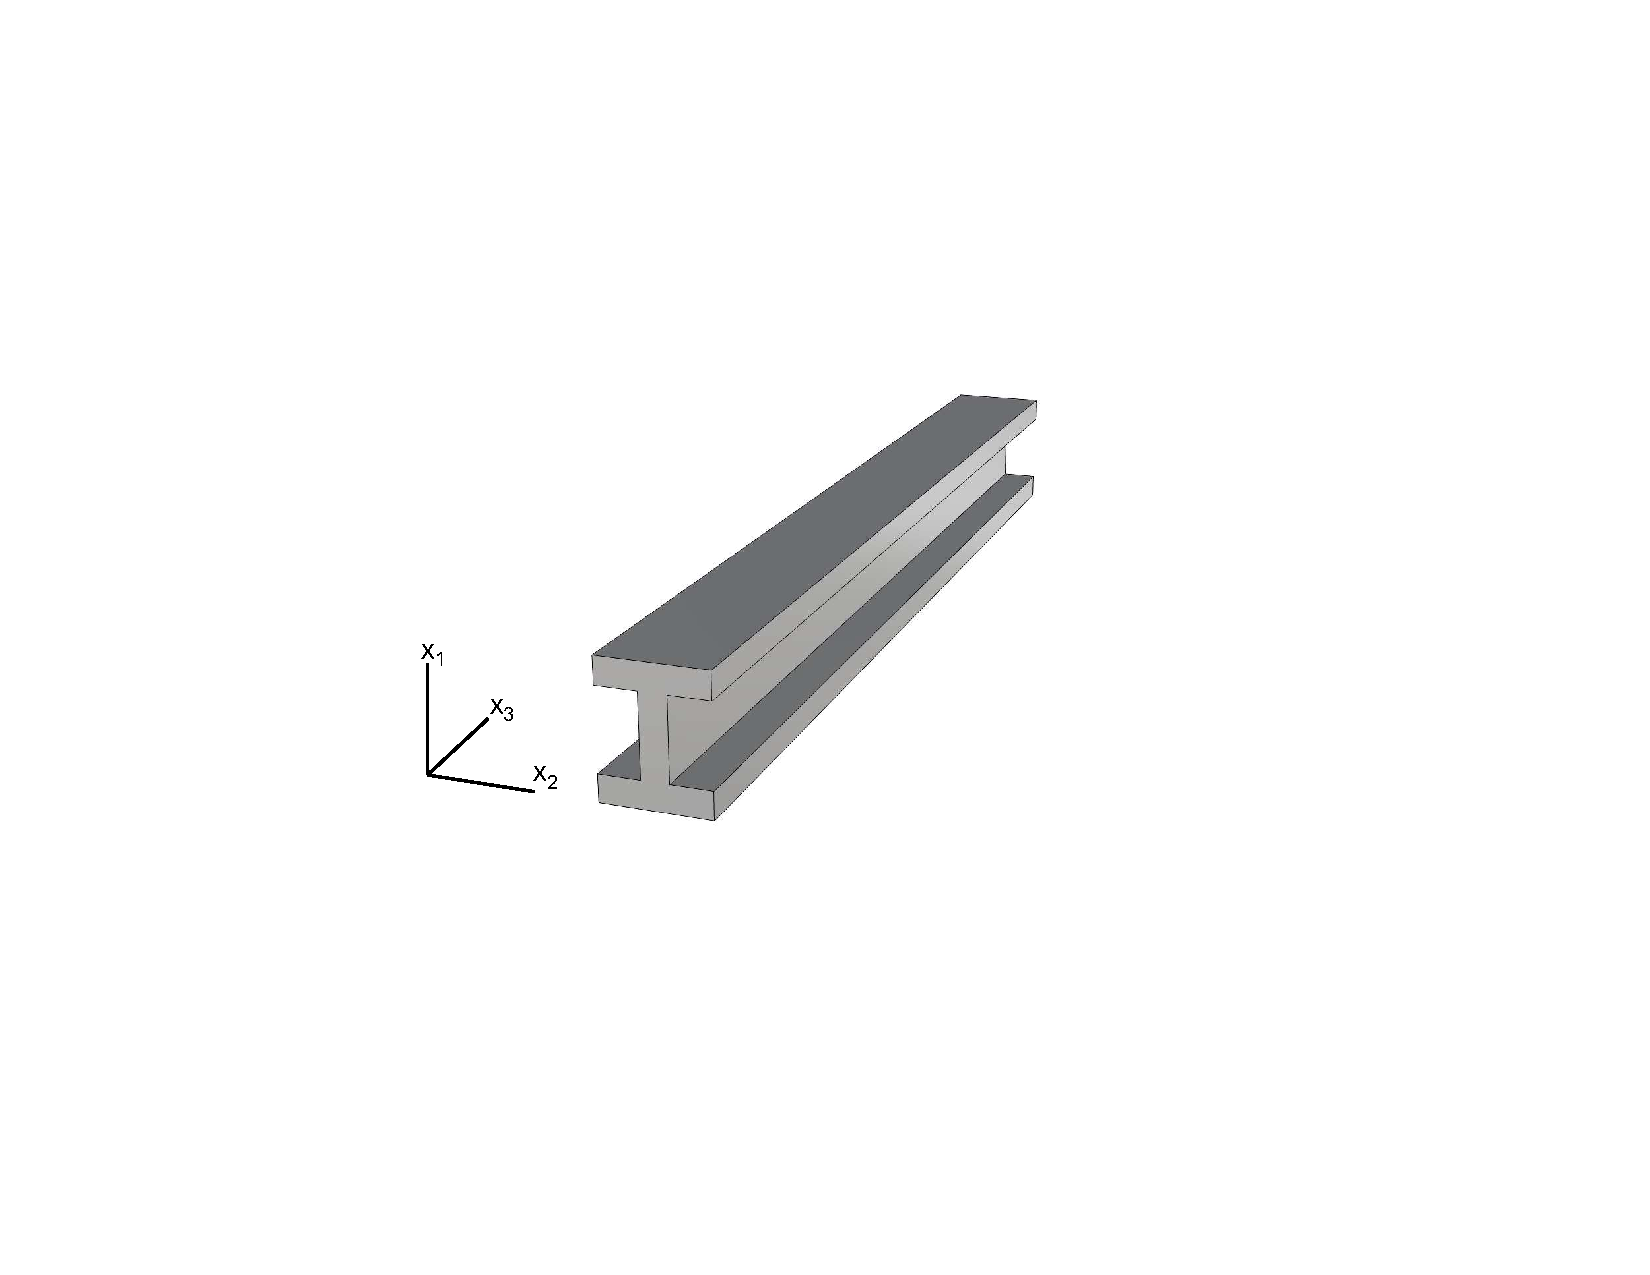
\includegraphics[width=0.2\columnwidth,trim=4cm 7cm 6cm 6.5cm, clip]{figs/straight.pdf}
}
\\
\subfloat[$\theta_1$]{
	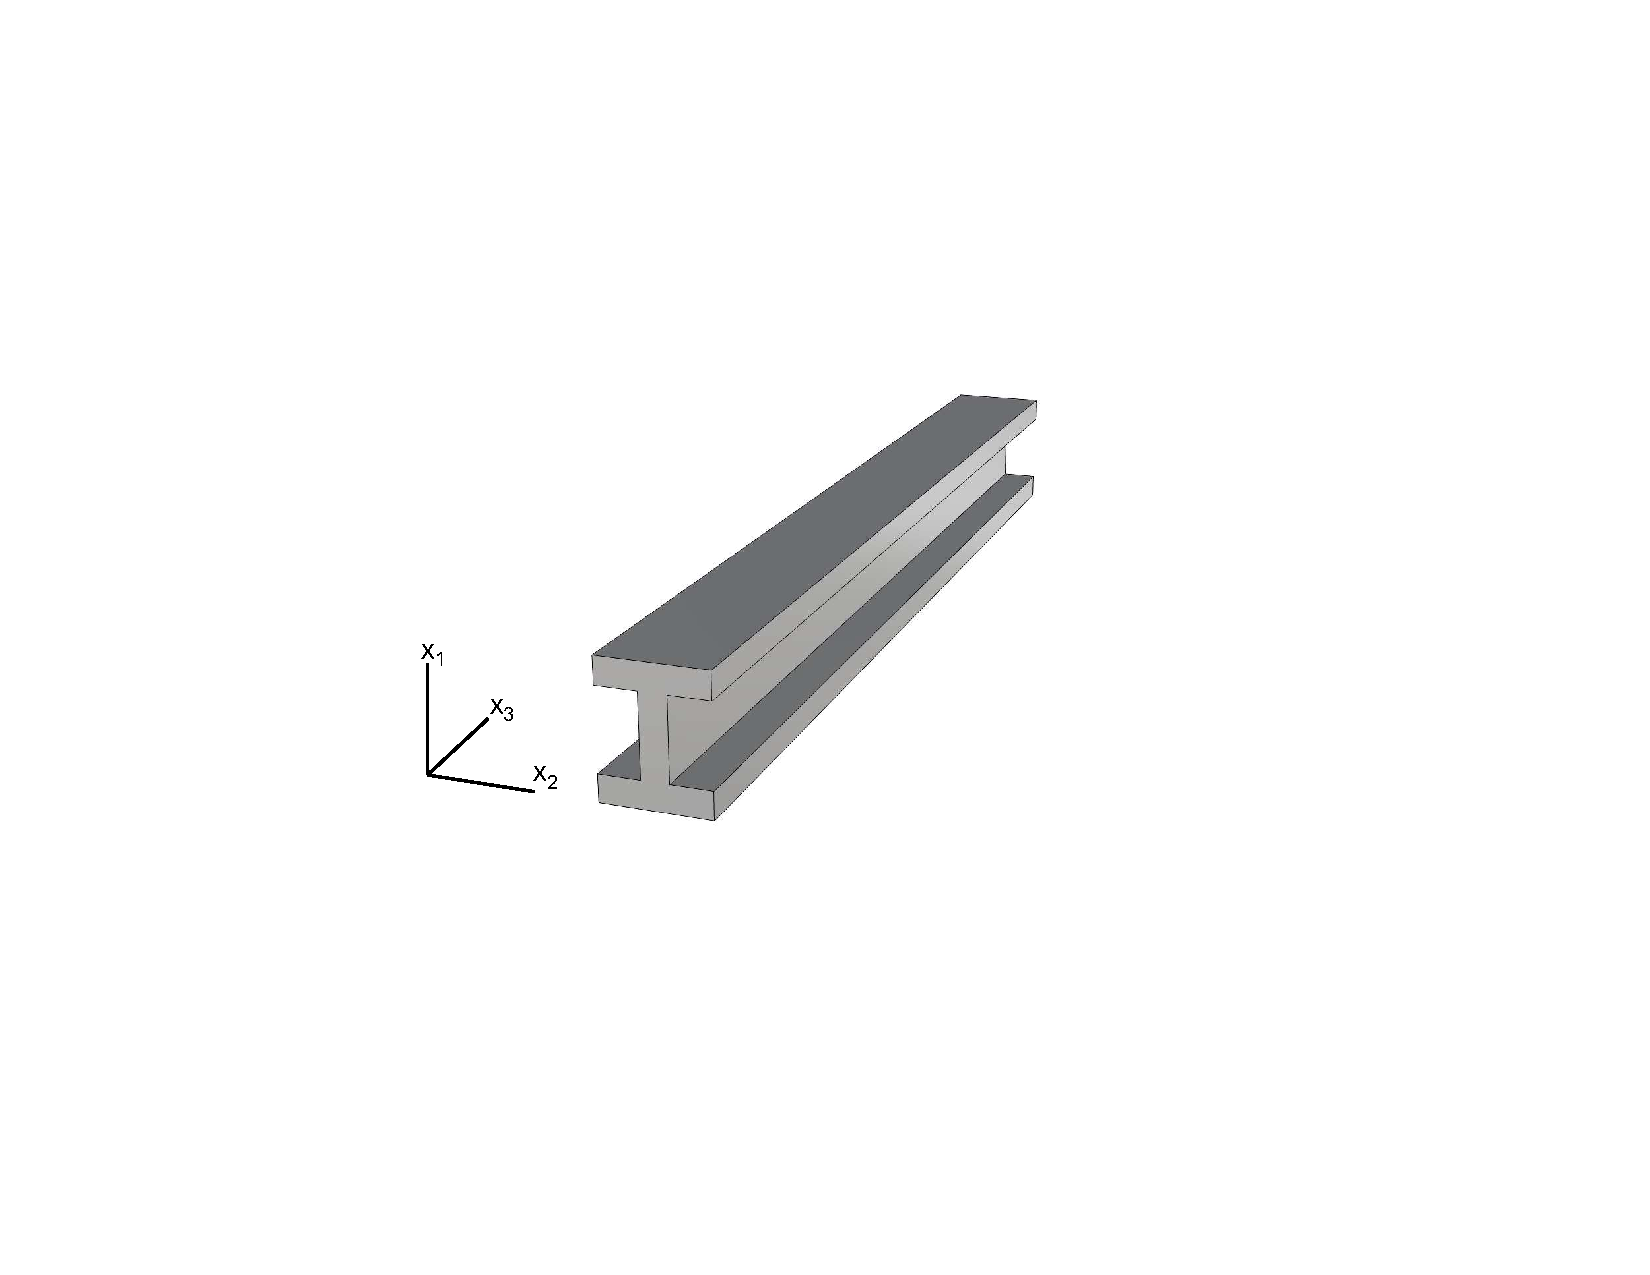
\includegraphics[width=0.2\columnwidth,trim=4cm 7cm 6cm 6.5cm, clip]{figs/straight.pdf}
}
\subfloat[$\theta_2$]{
	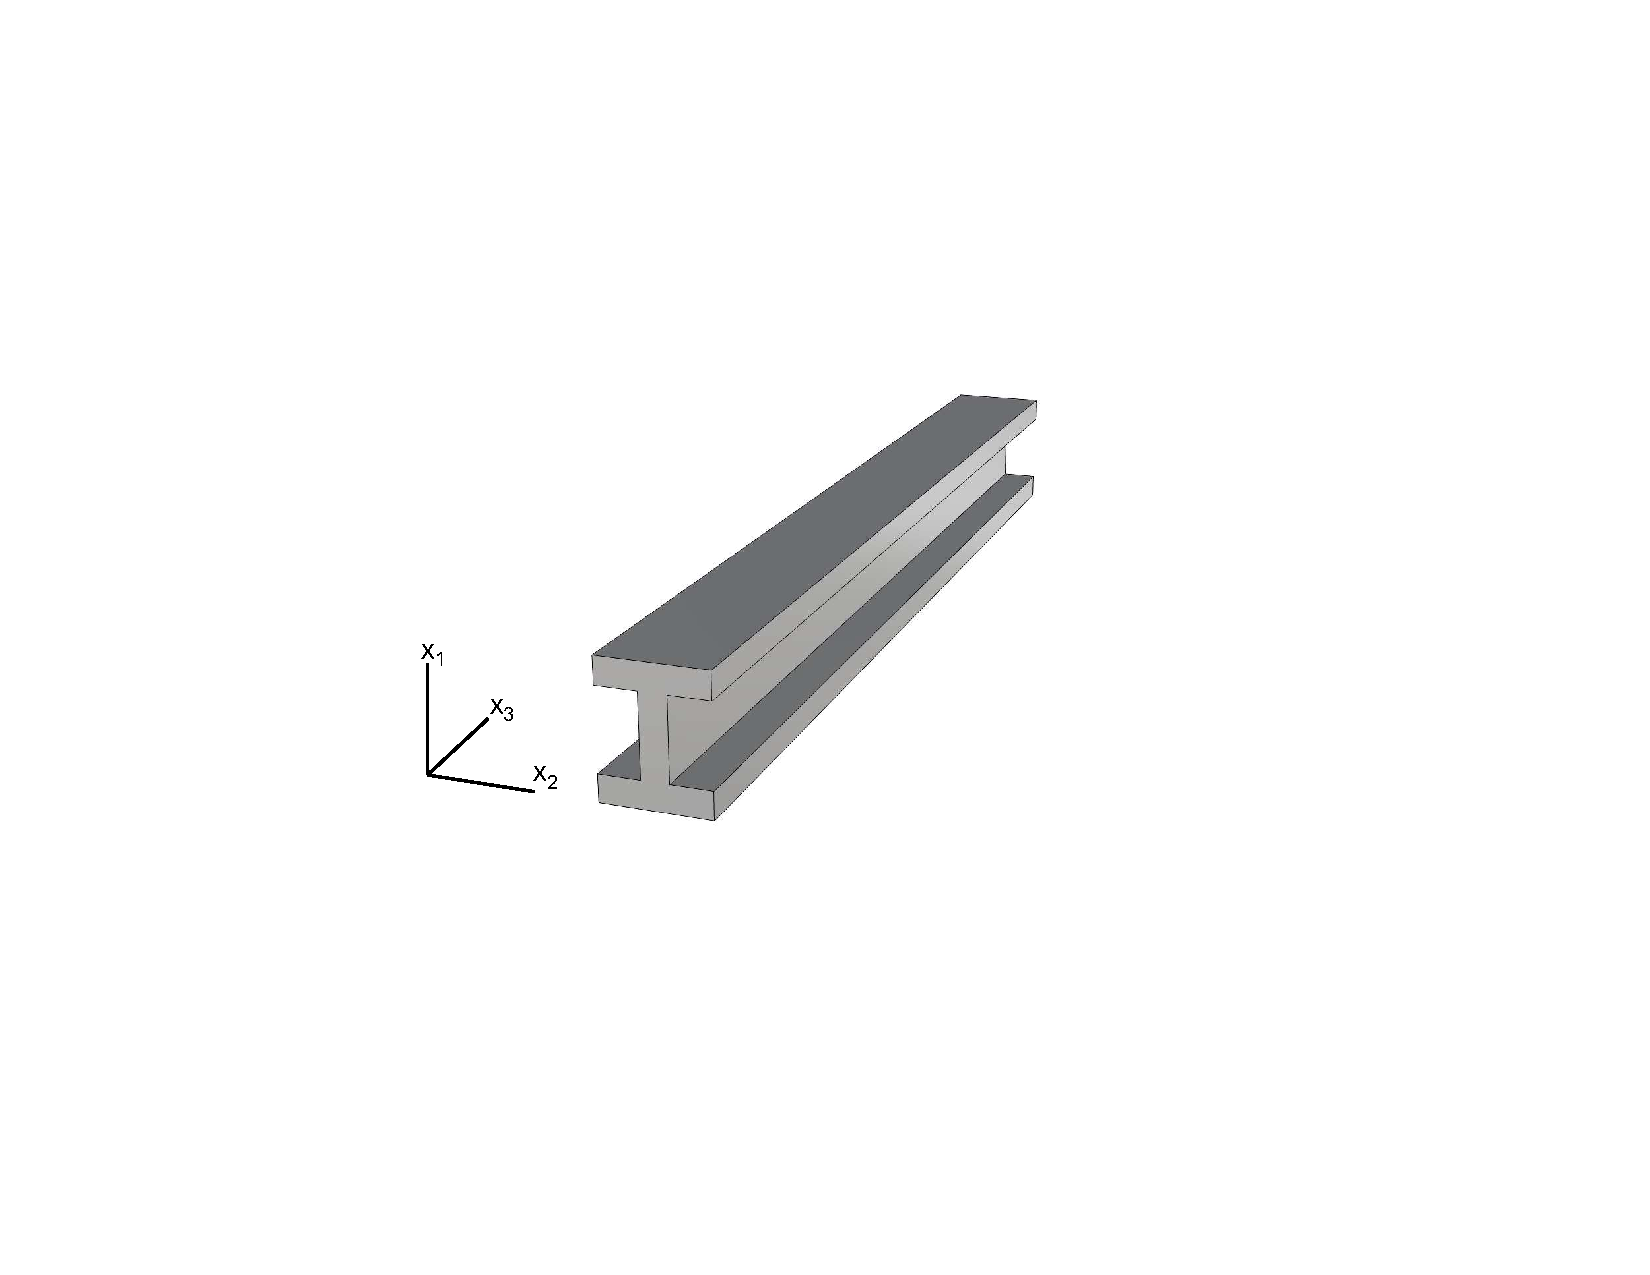
\includegraphics[width=0.2\columnwidth,trim=4cm 7cm 6cm 6.5cm, clip]{figs/straight.pdf}
}
\subfloat[$\theta_3$]{
	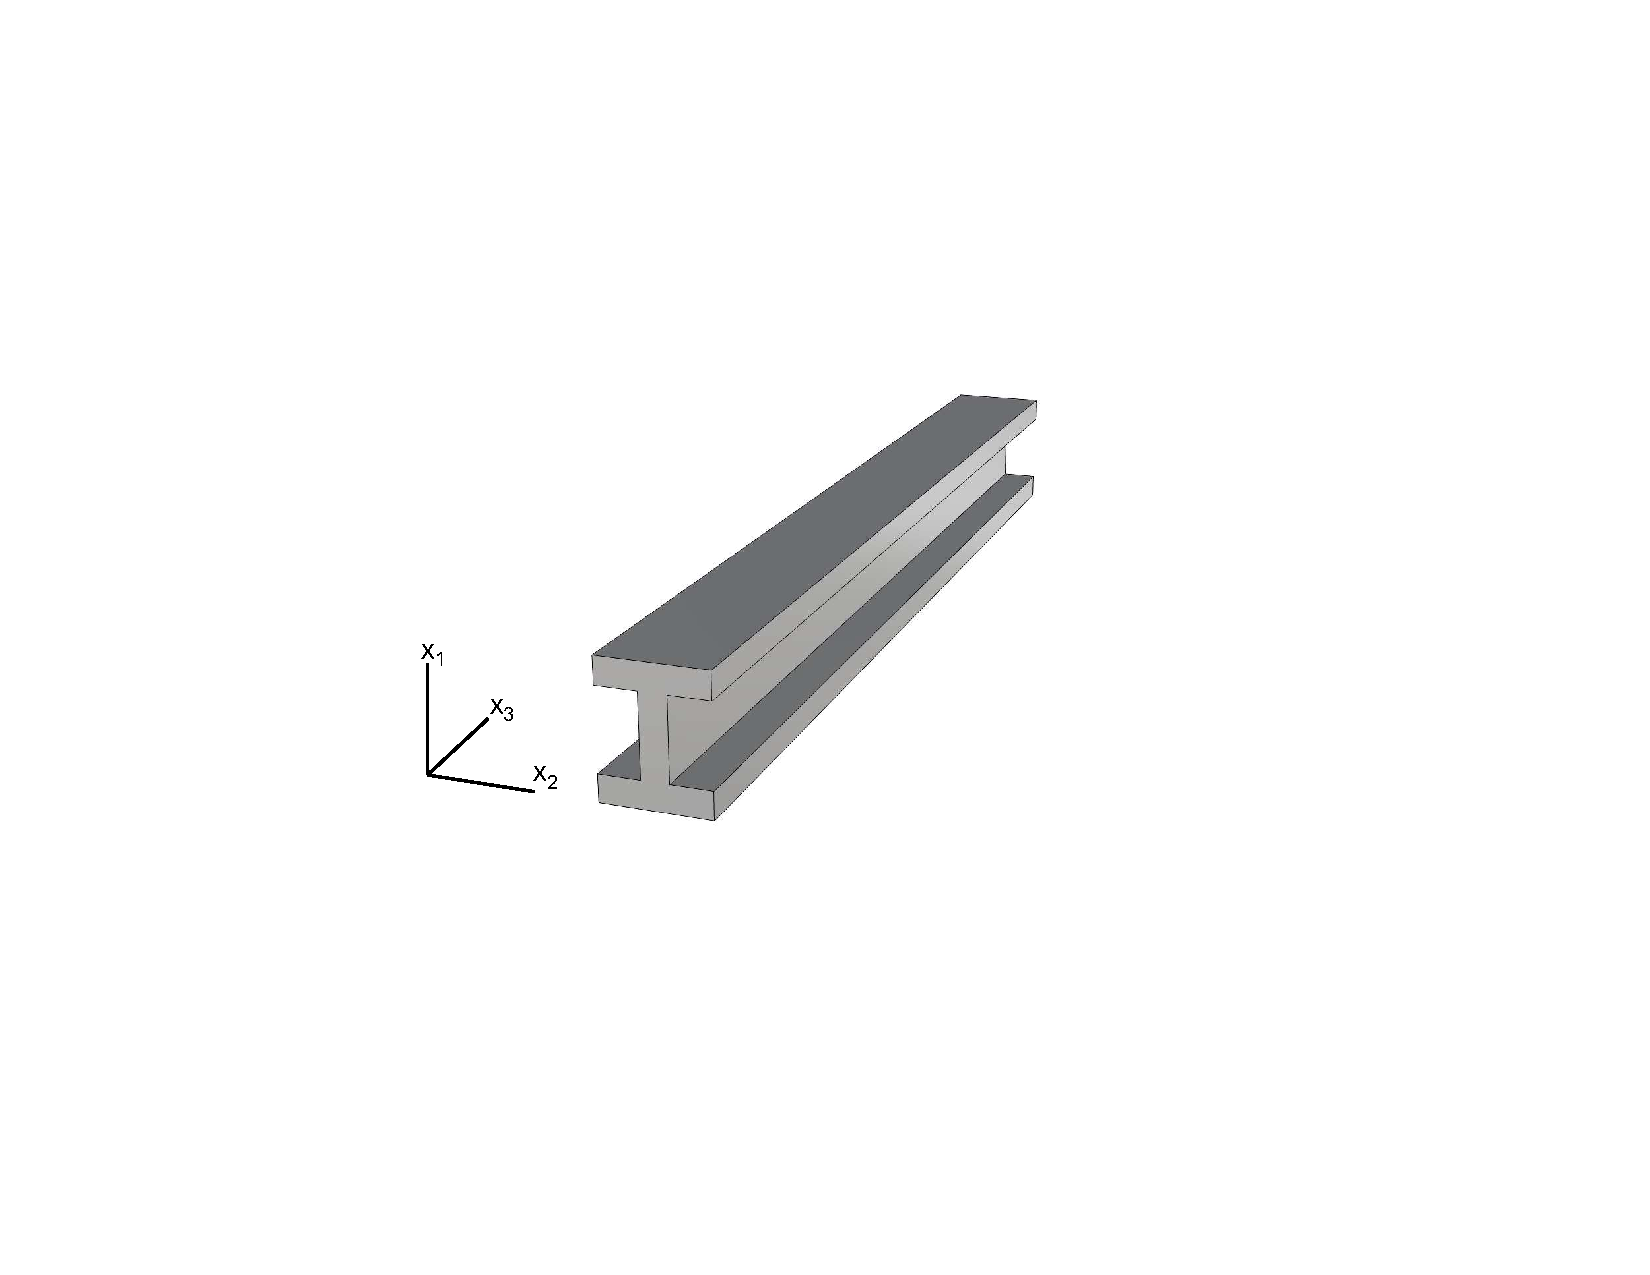
\includegraphics[width=0.2\columnwidth,trim=4cm 7cm 6cm 6.5cm, clip]{figs/straight.pdf}
}
\label{fig:w_theta_displacements}
\caption{Positive displacements in each coordinate direction for both translation and rotation are shown. CHANGE PICTURES}
\end{figure}

Note that in \cref{eq:u1} the $x_2\theta_3(x_3)$ term is subtracted $w_1(x_3)$, while in \cref{eq:u2} $x_1\theta_3(x_3)$ is added to $w_2(x_3)$.
This is an artifact of the positive/negative convection for rotation.
For a point $P$ at some positive valued $(x_1,x_2)$, the $u_1$ displacement is decreased by a $x_3$ rotation.
Similarly for the same point $P$, the $u_2$ displacement is increased by the $\theta_3$ rotation, see \cref{fig:u1u2_plus_minus_xtheta}.
The same sort of scenario occurs in \cref{eq:u3}, see \cref{fig:u3_plus_minus_xtheta}

\begin{figure}
\centering
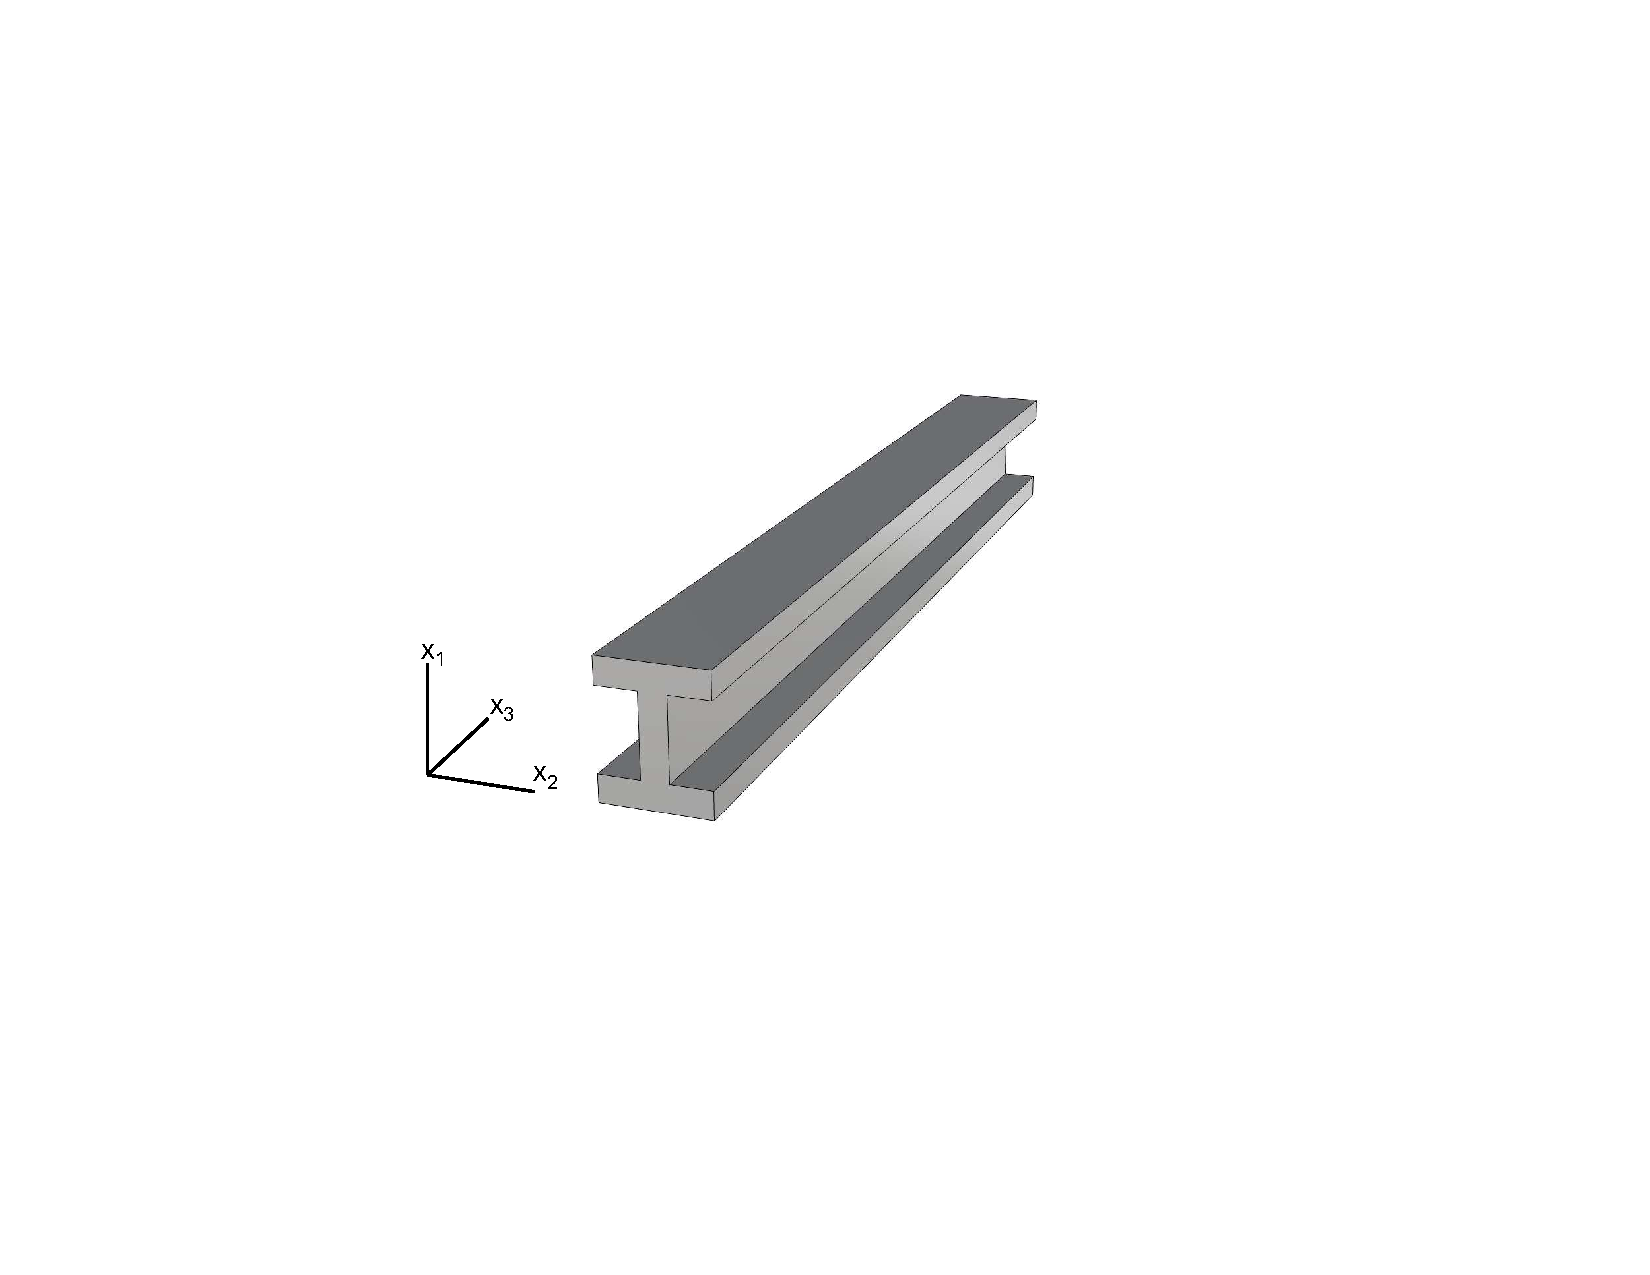
\includegraphics[width=0.2\columnwidth,trim=4cm 7cm 6cm 6.5cm, clip]{figs/straight.pdf}
\caption{A pictoral representation of sign convetion for $\theta_3$ rotations affecting $u_\alpha$ displacements. CHANGE PICTURE}
\label{fig:u1u2_plus_minus_xtheta}
\end{figure}

\begin{figure}
\centering
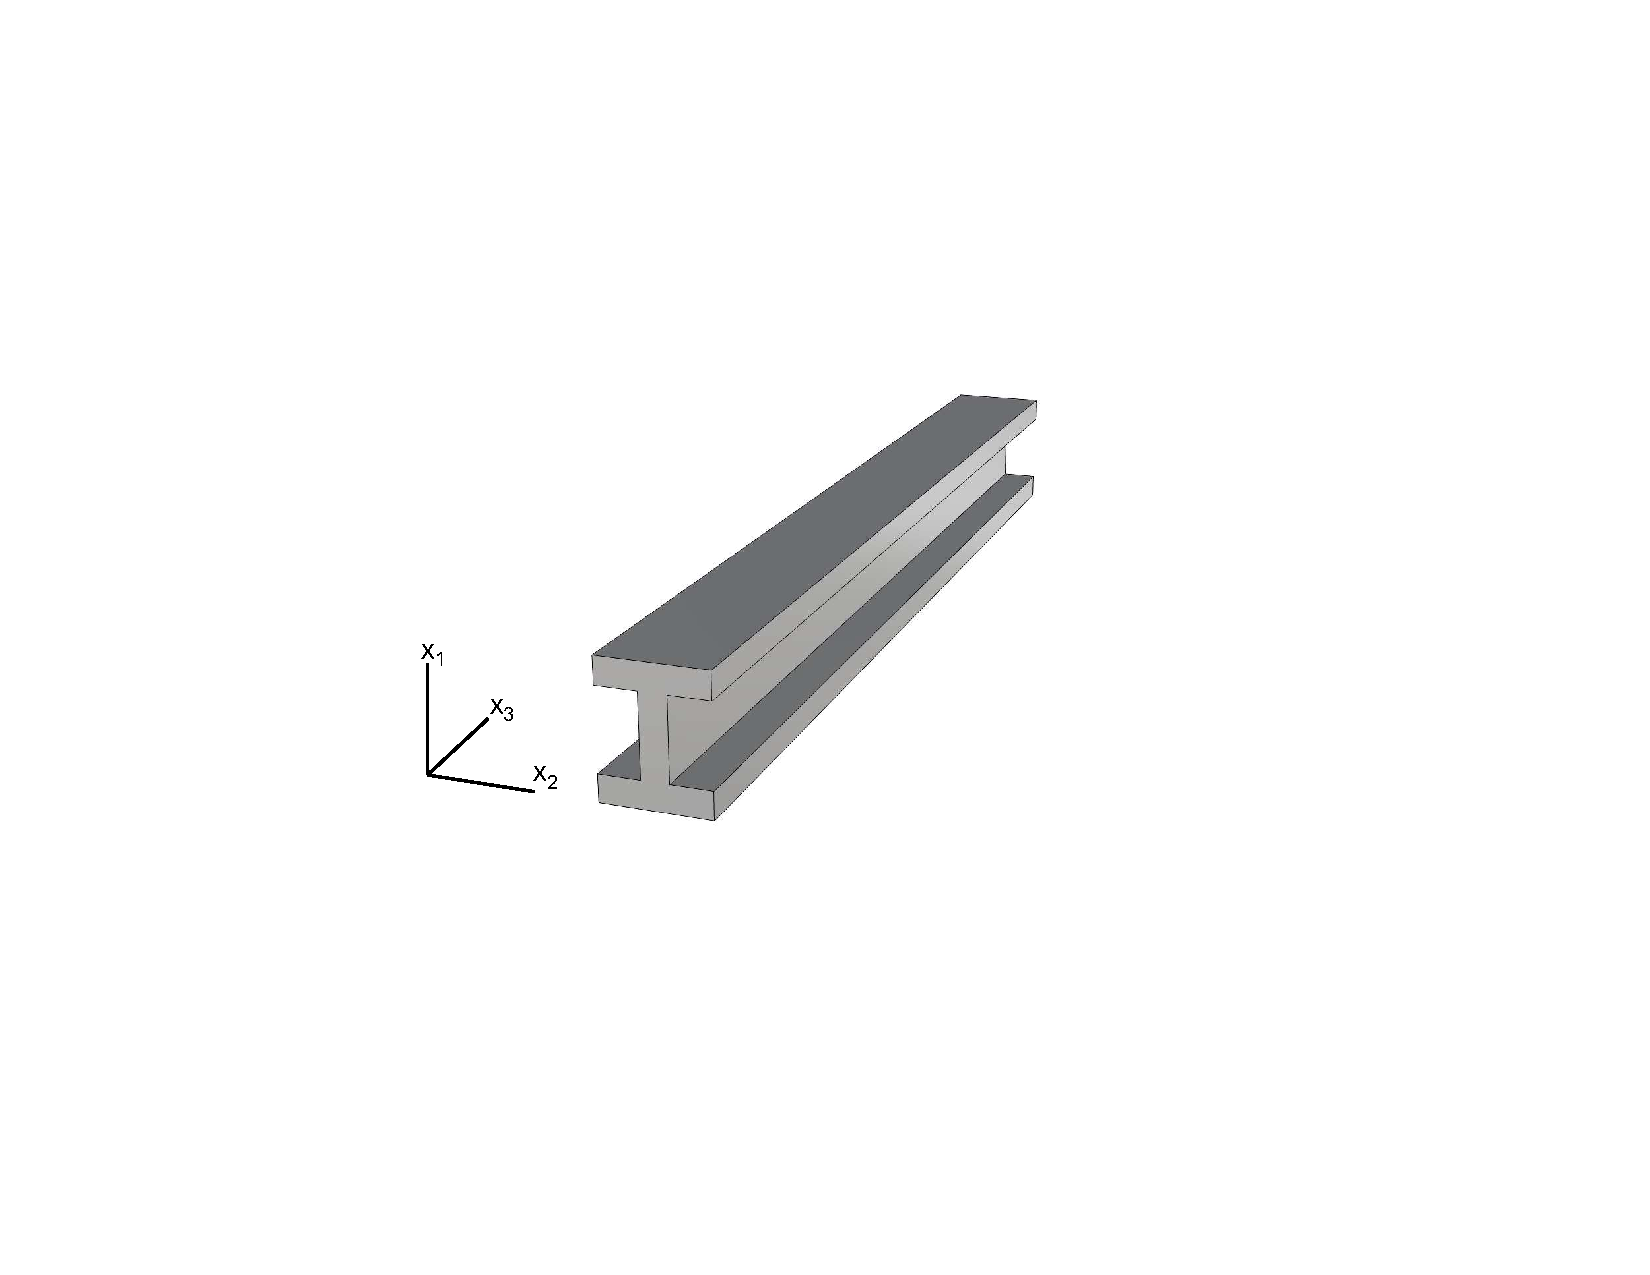
\includegraphics[width=0.2\columnwidth,trim=4cm 7cm 6cm 6.5cm, clip]{figs/straight.pdf}
\caption{A pictoral representation of sign convetion for $\theta_\alpha$ rotations affecting $u_3$ displacements. CHANGE PICTURE}
\label{fig:u3_plus_minus_xtheta}
\end{figure}

It is important to note that the anlysis will be limited or enhanced by the accuracy of these equations.
In this case, warping in the beam is not accounted for.

\subsection{Elastic Deformation}
All deformation in the beam is assumed to be elastic, as opposed to plastic.
Furthermore, we assume that the beam is homogeneous and isotropic.
This leads us to the special case for defining the stress tensor as \cref{eq:special_hookes}, where $\lambda$ and $\mu$ are Lame\'e constants describing material properties.

\begin{equation}
\sigma_{ij}=\lambda\delta_{ij}\epsilon_{kk}+2\mu\epsilon_{ij}
\label{eq:special_hookes}
\end{equation}


\subsection{Small Displacements}
As is customary in elastic methods, it is assumed that only small displacements occur.
